\documentclass[11pt]{article}
\usepackage{myz310e-notes}
\hypersetup{pdftitle={Convolutional networks: local connectivity, weight sharing and pooling},pdfauthor={Emre Onur Kahya},pdfsubject={MYZ 310E Machine Learning in Physics, Fall 2026, lecture note 13 (week 5)}}
\newcommand{\w}{\vect{w}}
\newcommand{\y}{\vect{y}}
\newcommand{\vdelta}{\vect{\delta}}
\newcommand{\Cin}{C_{\mathrm{in}}}
\newcommand{\Cout}{C_{\mathrm{out}}}
\newcommand{\Hout}{H'}
\newcommand{\Wout}{W'}
\newcommand{\ReLU}{\operatorname{ReLU}}
\renewcommand{\floatpagefraction}{0.75}
\usepackage{needspace}

\begin{document}
\NoteTitle{13}{5}{Convolutional networks:\\ local connectivity, weight sharing and pooling}{Convolutional networks}{%
A multilayer perceptron treats its input as an unordered list of numbers. Images, spectra, time series and lattice
configurations are not unordered: neighbouring values are related, and the same pattern may appear anywhere.
Convolutional networks build these two facts into the architecture. Each hidden unit looks only at a small patch
(\emph{local connectivity}), all units of a feature map use the same weights (\emph{parameter sharing}), and
\emph{pooling} summarises small neighbourhoods. This note derives the discrete convolution and its gradients, assembles
a complete network, shows how data augmentation supplies the invariances that the architecture lacks, follows the
architectures from AlexNet to residual networks, and then works out the arithmetic of convolutions --- output sizes,
padding, strides, dilation, convolution as a sparse matrix, and the transposed convolutions used to produce images as
outputs. Every operation comes with pseudocode and its cost.}

\section{Images and the three ideas}\label{sec:images}

The goal of \emph{object recognition} is to say which object an image contains. An image of height $H$ and width $W$
with $C$ colour channels is an array of $C \times H \times W$ numbers: $C = 1$ for a grey-scale image, $C = 3$ for red,
green and blue. Read as a vector, as in Note~1, Section~3, a $28 \times 28$ grey-scale digit gives $784$ inputs and a
modest $128 \times 128$ colour image $d = 3 \times 16\,384 = 49\,152$. Three properties distinguish such an input from a generic vector.

\begin{enumerate}
\item \emph{It is high-dimensional.} A fully connected hidden layer with $m$ units has $m(d + 1)$ parameters. For the
  $224 \times 224 \times 3$ images used on ImageNet ($d = 150\,528$), a single layer of 1000 hidden units already needs
  about $1.5 \times 10^8$ weights.
\item \emph{It has a topology.} Pixels sit on a two-dimensional grid (three-dimensional for video or volumetric
  data, one-dimensional for audio or a spectrum), and nearby pixels are strongly correlated. A fully connected layer
  ignores this: permuting the pixels of every image in the same way would not change what it can learn.
\item \emph{Its meaning is invariant under some transformations.} A cat shifted by ten pixels, slightly rotated or
  photographed in dimmer light is still a cat. Note~3, Section~4, listed such invariances as one reason why learning
  in very high dimension is possible at all, and Note~1, Section~3, showed with a three-pixel bar how badly raw pixel
  distances handle a one-pixel shift.
\end{enumerate}

Convolutional networks (\emph{convnets}, CNNs)~\cite{lecun1989,lecun1998} exploit these properties with three ideas,
which structure the first part of this note: \emph{local connectivity} (Section~\ref{sec:sharing}), \emph{parameter
sharing} (Sections~\ref{sec:sharing} and~\ref{sec:conv}) and \emph{pooling} (Section~\ref{sec:pool}). The rest of the
machinery --- neurons, activation functions, layers, the softmax output and the cross-entropy loss --- is that of the
multilayer perceptron of Note~11, Section~4, and the gradients are computed by backpropagation, Note~12, Section~3. A convnet is an MLP with
most of its weights forced to be zero and the remaining ones forced to be equal.

\section{Local connectivity and parameter sharing}\label{sec:sharing}

\paragraph{Local connectivity} Connect each hidden unit only to a small patch of the input, its \emph{receptive
field}, for instance a $3 \times 3$ or $5 \times 5$ square of pixels. The patch covers \emph{all} channels: a unit looking
at a $5 \times 5$ patch of a colour image has $5 \times 5 \times 3 = 75$ weights. Units at different positions look at
different patches, so together they tile the image. The idea comes from neuroscience: Hubel and Wiesel found that
neurons in the primary visual cortex of the cat respond to stimuli in a small region of the visual field, many of them to
edges of a particular orientation~\cite{hubel1962}, and Fukushima's neocognitron already stacked such local
units~\cite{fukushima1980}.

\paragraph{Parameter sharing} Go one step further and give all units that look for the same kind of pattern \emph{the
same} weights, wherever their patch lies. Such a group of units forms a \emph{feature map}: a two-dimensional grid of
units, one per position, all computing the same function of their own patch. A layer has several feature maps (also
called \emph{channels}), each with its own weights, so that one map may respond to vertical edges, another to
horizontal ones, a third to a colour contrast. Figure~\ref{fig:connect} contrasts the three kinds of layer in one
dimension.

\begin{figure}[htbp]
\centering
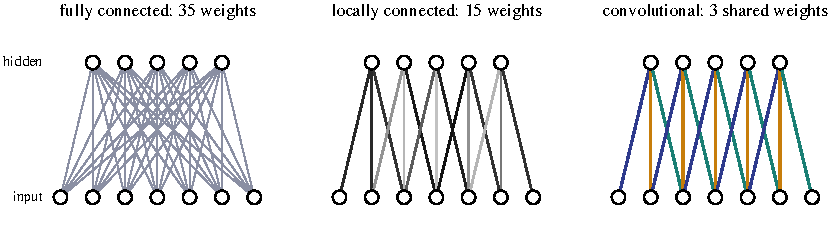
\includegraphics[width=\linewidth]{figures/n13_connectivity.pdf}
\caption{Three layers from seven inputs to five hidden units. Left: every unit sees every input. Centre: each unit
sees three neighbouring inputs with its own weights (grey levels). Right: each unit sees three neighbouring inputs and
all units use the same three weights (one colour per weight): a convolution.}
\label{fig:connect}
\end{figure}

\begin{worked}{1. Counting weights}
Take a $32 \times 32$ grey-scale image and a hidden layer with one unit per position of a $30 \times 30$ grid (the
positions where a $3 \times 3$ patch fits inside the image); ignore biases.
\begin{itemize}
\item \emph{Fully connected:} each of the $900$ units sees all $1024$ pixels: $900 \times 1024 = 921\,600$ weights.
\item \emph{Locally connected:} each unit sees its own $3 \times 3$ patch with its own weights: $900 \times 9 = 8100$
  weights.
\item \emph{Shared:} all units use the same $3 \times 3$ weights: $9$ weights, whatever the size of the image.
\end{itemize}
With 64 feature maps instead of one, the shared layer has $64 \times 9 = 576$ weights and the fully connected layer
$64 \times 921\,600 \approx 5.9 \times 10^7$. The computation shrinks less than the parameter count: the shared layer still
evaluates $900 \times 9$ multiply--adds per map, as many as the locally connected one. Sharing saves \emph{parameters}
(and hence data and memory); locality saves both parameters and \emph{operations}.
\end{worked}

\paragraph{What sharing buys} Fewer parameters mean less data needed to fit them, and a feature detector learned at one
position is immediately available at all others. Sharing also makes the layer \emph{equivariant} to translations: shift
the input, and every feature map shifts by the same amount, as Section~\ref{sec:equiv} proves. The two assumptions are
a prior about the data (Note~4, Section~7.3): local statistics matter, and they are the same everywhere. When this is false
--- the input is a table of unrelated measurements, or the absolute position carries the meaning --- convolutions are the
wrong tool.

\section{Discrete convolution}\label{sec:conv}

\subsection{One dimension}

Spatial indices start at $0$ in this note, channel indices at $1$. Let $x_0, \dots, x_{i-1}$ be a signal of length $i$ and $w_0, \dots, w_{k-1}$ a
\emph{kernel} (or filter) of size $k$. The unit at position $j$ of a shared, locally connected layer computes the
\emph{cross-correlation}
\begin{equation}\label{eq:xcorr1}
  y_j = (x \star w)_j = \sum_{m=0}^{k-1} w_m\, x_{j+m}, \qquad j = 0, 1, \dots, i - k ,
\end{equation}
a weighted sum of the window $x_j, \dots, x_{j+k-1}$ that slides along the signal. The output has $o = i - k + 1$
entries, one for each position where the window fits entirely inside the signal. The \emph{convolution} of signal
processing and physics,
\begin{equation}\label{eq:conv1}
  (x * w)_j = \sum_m w_m\, x_{j-m},
\end{equation}
runs through the kernel backwards. Restricted to the positions where the kernel fits, it equals the cross-correlation
with the flipped kernel $\tilde w_m = w_{k-1-m}$, up to an index shift: substituting $m' = k - 1 - m$,
\[
  (x \star \tilde w)_j = \sum_{m=0}^{k-1} w_{k-1-m}\, x_{j+m} = \sum_{m'=0}^{k-1} w_{m'}\, x_{j+k-1-m'} = (x * w)_{j+k-1} ,
\]
so the valid outputs of the true convolution carry the indices $j = k - 1, \dots, i - 1$ instead of $0, \dots, i - k$. Since the weights are learned, the flip is immaterial: a network that
needs $w$ in one convention learns $\tilde w$ in the other. Deep-learning libraries implement \eqref{eq:xcorr1} and
call it convolution, and so shall we from now on. The flip matters only when hand-designed kernels are compared or
when the mathematical properties of convolution are used: convolution is commutative and associative, cross-correlation
is not.

\begin{worked}{2. A one-dimensional convolution by hand}
Take $x = (2, 3, 5, 4, 1)$ and $w = (1, 0, -1)$. The window has three entries, so the output has $5 - 3 + 1 = 3$ entries:
\[
  y_0 = 2 - 5 = -3, \qquad y_1 = 3 - 4 = -1, \qquad y_2 = 5 - 1 = 4 .
\]
Each output is $y_j = x_j - x_{j+2} = -2\,(x_{j+2} - x_j)/2$, minus twice the central-difference estimate of the slope at
$j + 1$: the kernel measures the local slope of the signal, with
a sign. The signal rises and then falls, and $y$ goes from negative to positive accordingly. The true convolution
\eqref{eq:conv1} uses the flipped kernel $(-1, 0, 1)$ and gives $(3, 1, -4)$, the negative --- for this antisymmetric
kernel the flip only changes the sign. With the kernel $w = (1, 2, 0)$, cross-correlation gives $(8, 13, 13)$ and
convolution $(11, 14, 9)$: in general the two differ by more than a sign.
\end{worked}

\subsection{Two dimensions and several channels}

For an image $x_{u,v}$ and a $k \times k$ kernel $w_{a,b}$,
\begin{equation}\label{eq:xcorr2}
  y_{u,v} = \sum_{a=0}^{k-1}\sum_{b=0}^{k-1} w_{a,b}\, x_{u+a,\,v+b} .
\end{equation}
A layer of a convnet maps $\Cin$ input channels to $\Cout$ output channels. Its weights form a four-index array
$W \in \R^{\Cout \times \Cin \times k \times k}$ and it has one bias $b_c$ per output channel:
\begin{equation}\label{eq:convlayer}
  z_{c,u,v} = b_c + \sum_{c'=1}^{\Cin} \sum_{a,b=0}^{k-1} W_{c,c',a,b}\; x_{c',\,u+a,\,v+b}, \qquad
  h_{c,u,v} = g(z_{c,u,v}) ,
\end{equation}
with an element-wise activation $g$ (ReLU in most modern networks, Note~11, Section~2; we write $z$, not $a$, for the
pre-activation, because $a, b$ index kernel offsets). Each output channel sums the
cross-correlations of \emph{all} input channels with its own slice $W_{c,c',\cdot,\cdot}$: a filter is a $\Cin \times k
\times k$ block, and the layer has
\begin{equation}\label{eq:params}
  \Cout\,(\Cin k^2 + 1) \quad \text{parameters,}
\end{equation}
independently of the image size. The first layer of AlexNet (Section~\ref{sec:history}), for example, has $96$ filters of
size $3 \times 11 \times 11$, that is $96 \times (363 + 1) = 34\,944$ parameters. The array $z$ is the
\emph{pre-activation feature map}, $h$ the feature map proper.

\begin{worked}{3. A two-dimensional convolution by hand}
Take the $4 \times 4$ image and the $3 \times 3$ kernel
\[
  x = \begin{pmatrix} 1 & 2 & 0 & 1 \\ 0 & 1 & 3 & 1 \\ 2 & 1 & 0 & 0 \\ 1 & 0 & 1 & 2 \end{pmatrix}, \qquad
  w = \begin{pmatrix} 1 & 0 & -1 \\ 1 & 0 & -1 \\ 1 & 0 & -1 \end{pmatrix}.
\]
The $3 \times 3$ window fits in $2 \times 2$ positions. With this kernel each output is the sum of the left column of the
window minus the sum of its right column. Top left (rows 0--2, columns 0--2): $(1 + 0 + 2) - (0 + 3 + 0) = 0$. Top right
(columns 1--3): $(2 + 1 + 1) - (1 + 1 + 0) = 2$. Bottom left (rows 1--3): $(0 + 2 + 1) - (3 + 0 + 1) = -1$. Bottom right:
$(1 + 1 + 0) - (1 + 0 + 2) = -1$. Hence
\[
  y = x \star w = \begin{pmatrix} 0 & 2 \\ -1 & -1 \end{pmatrix}, \qquad
  \ReLU(y + 1) = \begin{pmatrix} 1 & 3 \\ 0 & 0 \end{pmatrix}
\]
with a bias of $+1$. Surrounding the image by a border of zeros (\emph{zero padding}, Section~\ref{sec:arith}) keeps the
output at $4 \times 4$; moving the window two pixels at a time (\emph{stride} $2$) keeps only every second output. Both
are used in Question~B2.

\emph{Two input channels.} With $\Cin = 2$, one output channel sums the cross-correlations of both input channels with
their own slices of its filter, as in \eqref{eq:convlayer}. Take the $3 \times 3$ channels and $2 \times 2$ slices
\[
  x_1 = \begin{pmatrix} 1 & 2 & 0 \\ 0 & 1 & 3 \\ 2 & 1 & 0 \end{pmatrix}, \quad
  x_2 = \begin{pmatrix} 1 & 0 & 1 \\ 0 & 2 & 0 \\ 1 & 0 & 1 \end{pmatrix}, \quad
  W_{1,1} = \begin{pmatrix} 1 & 0 \\ 0 & 1 \end{pmatrix}, \quad
  W_{1,2} = \begin{pmatrix} 0 & 1 \\ 1 & 0 \end{pmatrix}.
\]
$W_{1,1}$ adds the diagonal of each window of $x_1$, $W_{1,2}$ the anti-diagonal of each window of $x_2$; with bias $b_1 = 1$,
\[
  z_{1} = \begin{pmatrix} 2 & 5 \\ 1 & 1 \end{pmatrix} + \begin{pmatrix} 0 & 3 \\ 3 & 0 \end{pmatrix} + 1
  = \begin{pmatrix} 3 & 9 \\ 5 & 2 \end{pmatrix} .
\]
A second output channel would repeat the computation with its own two slices.
\end{worked}

\subsection{Equivariance, and a convolution as a feature detector}\label{sec:equiv}

Let $(T_s x)_j = x_{j - s}$ shift a signal by $s$ positions (for an infinite signal, or away from the borders). Then
\[
  \big((T_s x) \star w\big)_j = \sum_m w_m\, x_{j + m - s} = (x \star w)_{j - s} = \big(T_s(x \star w)\big)_j :
\]
shifting the input and then convolving gives the same as convolving and then shifting. The convolution
\emph{commutes} with translations; it is \emph{translation equivariant}. The element-wise activation also commutes
with shifts, so a whole convolutional layer with stride $1$, and a stack of such layers, is equivariant (up to border
effects); a layer with stride $s$ is equivariant only to shifts by multiples of $s$ (compare Worked example~5). A function $f$
is \emph{invariant} if $f(T_s x) = f(x)$ instead; equivariant maps keep track of \emph{where} a pattern is, invariant
ones forget it. Classification needs invariance at the end; Section~\ref{sec:pool} shows how pooling turns equivariance
into approximate invariance.

\begin{worked}{4. An edge detector moves with the edge}
A $5 \times 5$ image is dark ($0$) in its two left columns and bright ($2$) elsewhere; every row is $(0, 0, 2, 2, 2)$.
The kernel with three identical rows $(-1, 0, 1)$ computes, at each window, (right column) $-$ (left column), summed over
three rows. Each row of the $3 \times 3$ output is $(3 \cdot 2,\ 3 \cdot 2,\ 0) = (6, 6, 0)$: large where the window
straddles the dark-to-bright step, zero where it lies in the uniform bright region. Shift the edge one column to the right,
so that every row reads $(0, 0, 0, 2, 2)$: every row of the output becomes $(0, 6, 6)$, the old response shifted by one
column. The detector does not need to know where the edge is; the position is encoded in \emph{which} output units
respond.
\end{worked}

Figure~\ref{fig:fmaps} applies two hand-made $3 \times 3$ edge filters, each followed by a ReLU, to a synthetic image. The
first map lights up along dark-to-bright transitions from left to right, the second along transitions from top to
bottom. Shifting the input by $(3, 4)$ pixels shifts the map by exactly $(3, 4)$ away from the borders, as the derivation
above requires. A trained convnet finds such filters by itself (Section~\ref{sec:history}).

\begin{figure}[htbp]
\centering
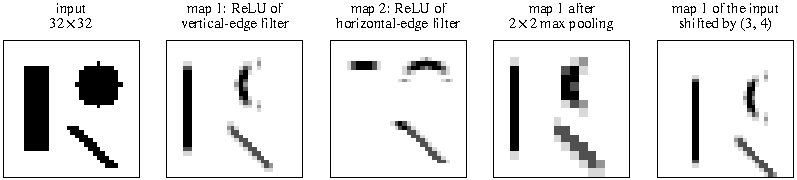
\includegraphics[width=\linewidth]{figures/n13_feature_maps.pdf}
\caption{Feature maps of a $32 \times 32$ synthetic image (zero padding, so maps keep the image size). Map~1 uses the
kernel with rows $(-1, 0, 1)$, $(-2, 0, 2)$, $(-1, 0, 1)$; map~2 its transpose. Fourth panel: map~1 after $2 \times 2$ max
pooling, $16 \times 16$. Last panel: map~1 of the image shifted by $3$ rows and $4$ columns; in the interior it equals the
second panel shifted by the same amounts.}
\label{fig:fmaps}
\end{figure}

\begin{algorithm}[htbp]
\caption{Convolutional layer, forward pass (direct form)}\label{alg:conv}
\begin{algorithmic}[1]
\Require input $x \in \R^{\Cin \times H \times W}$; weights $W \in \R^{\Cout \times \Cin \times k \times k}$; biases
  $\vect{b} \in \R^{\Cout}$; stride $s$; padding $p$; activation $g$
\Function{ConvForward}{$x$; $W, \vect{b}, s, p$}
  \State $\bar x \gets x$ surrounded by $p$ zeros on each side of each spatial axis \Comment{Section~\ref{sec:arith}}
  \State $\Hout \gets \lfloor (H + 2p - k)/s \rfloor + 1$; \ $\Wout \gets \lfloor (W + 2p - k)/s \rfloor + 1$
  \For{$c = 1, \dots, \Cout$; \ $u = 0, \dots, \Hout - 1$; \ $v = 0, \dots, \Wout - 1$}
    \State $z_{c,u,v} \gets b_c + \sum_{c'=1}^{\Cin}\sum_{a,b=0}^{k-1} W_{c,c',a,b}\; \bar x_{c',\,su+a,\,sv+b}$
      \Comment{$\Cin k^2$ multiply--adds}
  \EndFor
  \State $h \gets g(z)$ element-wise
  \State \Return $h$ (and keep $\bar x$, $z$ for the backward pass)
\EndFunction
\end{algorithmic}
\end{algorithm}

\begin{runtime}{convolutional layer, forward}
\emph{Time}: $O(\Cout\Hout\Wout\,\Cin k^2)$ multiply--adds per example: one dot product of length $\Cin k^2$ per output
unit. A $3 \times 3$ layer from 64 to 64 channels on a $56 \times 56$ map needs $56^2 \cdot 64 \cdot 64 \cdot 9 \approx
1.2 \times 10^8$ multiply--adds; a fully connected layer between the same two arrays would need $(56^2 \cdot 64)^2
\approx 4 \times 10^{10}$. \emph{Memory}: $\Cout(\Cin k^2 + 1)$ parameters ($36\,928$ in the example), plus the
$\Cout\Hout\Wout$ activations, which must be kept for the backward pass --- in deep convnets the activations, not the
weights, dominate memory during training. \emph{Prediction}: the same as the forward pass. Libraries do not run these
loops literally; Section~\ref{sec:arith} shows the matrix-product form they use.
\end{runtime}

\begin{physics}{shift symmetry, Green's functions and Fourier modes}
Physicists know convolutions as the response of linear, time-invariant systems: the output of a damped oscillator or
an RC circuit is the input convolved with the impulse response (the Green's function), and the field of a charge
distribution is the density convolved with the Coulomb kernel. This is no coincidence: any linear map on signals that
commutes with all translations is a convolution (Question~C1). Translation symmetry therefore fixes the \emph{form} of a
linear layer; learning only chooses the kernel. Like a translation-invariant Hamiltonian, such a map is diagonal in the
Fourier basis, which is the convolution theorem: $\widehat{x * w} = \hat x\,\hat w$. The same reasoning extends to other
symmetry groups. Group-equivariant CNNs share weights across rotations and reflections as well as
translations~\cite{cohen2016}, and networks for molecules and crystals are built to respect rotations and permutations of
identical atoms --- symmetry, not data, removes those degrees of freedom.
\end{physics}

\section{Pooling}\label{sec:pool}

The third idea is to summarise small neighbourhoods of each feature map. \emph{Max pooling} over $m \times m$ blocks with
stride $m$ (non-overlapping blocks) computes, separately for each channel $c$,
\begin{equation}\label{eq:maxpool}
  y_{c,u,v} = \max_{0 \le a, b < m}\ h_{c,\,mu + a,\,mv + b} ,
\end{equation}
and \emph{average pooling} replaces the maximum by the mean $\frac{1}{m^2}\sum_{a,b} h_{c,\,mu+a,\,mv+b}$. Pooling has no
parameters, acts on each channel separately, and with $m = 2$ divides the height and the width by two, the number of
units by four. Overlapping windows (window $3$, stride $2$, as in AlexNet) are also used.

Pooling does two things. It \emph{subsamples}: later layers see a coarser grid and cost less. And it buys \emph{local
invariance}: the maximum of a block does not change when its largest entry moves within the block.

\begin{worked}{5. Max pooling and small shifts}
Pool the $4 \times 4$ feature map $h$ in $2 \times 2$ blocks:
\[
  h = \begin{pmatrix} 6 & 0 & 2 & 0 \\ 1 & 0 & 0 & 1 \\ 0 & 0 & 4 & 0 \\ 3 & 0 & 1 & 0 \end{pmatrix}
  \ \longmapsto\ \begin{pmatrix} 6 & 2 \\ 3 & 4 \end{pmatrix}
  \qquad(\text{average pooling: } \begin{pmatrix} 1.75 & 0.75 \\ 0.75 & 1.25 \end{pmatrix}).
\]
Shift $h$ to the right by one or by two columns, filling with zeros, and pool again:
\[
  \text{shift by 1: } \begin{pmatrix} 6 & 2 \\ 3 & 4 \end{pmatrix}, \qquad
  \text{shift by 2: } \begin{pmatrix} 0 & 6 \\ 0 & 3 \end{pmatrix} .
\]
After a shift by one, every maximum moves from the left column of its block to the right column of the same block, and
the pooled map is unchanged: invariant. After a shift by two the maxima cross into the next block, and the result is the
old pooled map shifted by one cell (its right column has left the image). A shift by a multiple of the pooling stride is reproduced, on the coarser grid, as a shift; smaller shifts are
absorbed only when they do not carry a maximum across a block boundary. Pooling gives approximate, local invariance, not
an exact one.
\end{worked}

\paragraph{Gradients through pooling} Backpropagation (Note~12, Section~3) needs $\partial y/\partial h$. For max pooling, $y_{c,u,v}$
equals one entry of its block and does not depend on the others (where the maximum is unique), so the incoming gradient
is routed entirely to the position of the maximum, the \emph{argmax}, and the other entries of the block receive zero.
For average pooling every entry of the block receives $1/m^2$ of it.

\begin{algorithm}[htbp]
\caption{Max pooling ($m \times m$ blocks, stride $m$): forward and backward}\label{alg:pool}
\begin{algorithmic}[1]
\Require feature maps $h \in \R^{C \times H \times W}$ with $H, W$ divisible by $m$
\Function{MaxPoolForward}{$h$; $m$}
  \For{$c = 1, \dots, C$; \ $u = 0, \dots, H/m - 1$; \ $v = 0, \dots, W/m - 1$}
    \State $(a^*, b^*) \gets \argmax_{0 \le a, b < m} h_{c,\,mu+a,\,mv+b}$; \ $y_{c,u,v} \gets h_{c,\,mu+a^*,\,mv+b^*}$
    \State store $(a^*, b^*)$ as $\mathrm{arg}_{c,u,v}$ \Comment{needed by the backward pass}
  \EndFor
  \State \Return $y$, $\mathrm{arg}$
\EndFunction
\Function{MaxPoolBackward}{$\partial \ell/\partial y$, $\mathrm{arg}$; $m$}
  \State $\bar h \gets$ zero array of the shape of $h$
  \For{each $(c, u, v)$, with $(a^*, b^*) = \mathrm{arg}_{c,u,v}$}
    \State $\bar h_{c,\,mu+a^*,\,mv+b^*} \gets \partial \ell/\partial y_{c,u,v}$ \Comment{gradient goes to the winner only}
  \EndFor
  \State \Return $\bar h = \partial \ell/\partial h$
\EndFunction
\Statex \textsc{AvgPoolBackward}: $\bar h_{c,\,mu+a,\,mv+b} \gets \frac{1}{m^2}\,\partial \ell/\partial y_{c,u,v}$ for all $0 \le a, b < m$
\end{algorithmic}
\end{algorithm}

\begin{runtime}{pooling}
\emph{Time}: $O(CHW)$ per example for both passes, since every input entry is compared (or added) once; this is small
next to the convolutions. \emph{Memory}: no parameters; the output has $CHW/m^2$ entries, and the forward pass stores
one argmax index per output for training. Pooling divides the cost of every later layer by $m^2$. Global average
pooling (Section~\ref{sec:arith}) is the case $m = H = W$, at cost $O(CHW)$.
\end{runtime}

\begin{physics}{pooling and coarse-graining}
Kadanoff's block-spin construction replaces each $3 \times 3$ block of Ising spins by one spin, for instance by majority
rule, and asks how the couplings change under this coarse-graining; iterating it is a real-space renormalisation-group
transformation. A stack of convolutions and pooling layers is reminiscent of this: local operations followed by
subsampling, with fine detail discarded and large-scale structure kept. Mehta and Schwab made the analogy precise for one
particular model class, mapping variational renormalisation onto stacked restricted Boltzmann
machines~\cite{mehta2014}. It should be read as an analogy, not an identity: the renormalisation group keeps what
determines long-distance physics, while a classifier keeps whatever predicts its label. Note also that pooling, like
block-spin averaging, cannot be undone --- a fact that matters when an image must be produced as output
(Section~\ref{sec:transposed}).
\end{physics}

\section{A complete convolutional network}\label{sec:convnet}

A convolutional network alternates convolutional layers (with their activation) and pooling layers. The number of
channels usually grows as the spatial size shrinks, so that each stage trades resolution for more kinds of features. At
the end the remaining feature maps are flattened into a vector, or averaged over positions (Section~\ref{sec:arith}),
and fed to one or more fully connected layers and a softmax output exactly as in an MLP (Note~11, Sections~4 and~5). This is the design of
LeNet~\cite{lecun1998}, which read handwritten digits on bank cheques in the 1990s, and in outline of every convnet since.

\needspace{14\baselineskip}
\begin{worked}{6. Shapes and parameters of a LeNet-style network}
Input: a $1 \times 28 \times 28$ grey-scale digit; ten classes. Convolutions have stride $1$ and ReLU activations,
pooling is $2 \times 2$ max pooling. Shapes are written channels $\times$ height $\times$ width; ``multiply--adds'' counts
the forward pass for one image.
\begin{center}\small
\begin{tabular}{@{}lllrr@{}}
\toprule
layer & operation & output shape & parameters & multiply--adds \\
\midrule
conv 1 & $6$ filters $1 \times 5 \times 5$, $p = 2$ & $6 \times 28 \times 28$ & $156$ & $117\,600$ \\
pool 1 & $2 \times 2$ max & $6 \times 14 \times 14$ & $0$ & --- \\
conv 2 & $16$ filters $6 \times 5 \times 5$, $p = 0$ & $16 \times 10 \times 10$ & $2\,416$ & $240\,000$ \\
pool 2 & $2 \times 2$ max & $16 \times 5 \times 5 = 400$ & $0$ & --- \\
fc 1 & $400 \to 120$ & $120$ & $48\,120$ & $48\,000$ \\
fc 2 & $120 \to 84$ & $84$ & $10\,164$ & $10\,080$ \\
fc 3 + softmax & $84 \to 10$ & $10$ & $850$ & $840$ \\
\midrule
total & & & $61\,706$ & $416\,520$ \\
\bottomrule
\end{tabular}
\end{center}
By \eqref{eq:params}, conv~1 has $6(25 + 1) = 156$ parameters and conv~2 has $16(150 + 1) = 2\,416$. Two features of convnets are visible. The convolutions hold $4\%$ of the parameters but do $86\%$ of the computation
(each weight is reused at hundreds of positions), while the first fully connected layer holds most of the parameters.
And a fully connected layer producing the same $6 \times 28 \times 28$ output as conv~1 would need
$784 \times 4704 + 4704 = 3\,692\,640$ parameters instead of $156$.
\end{worked}

\paragraph{The receptive field grows with depth} A unit of conv~1 sees a $5 \times 5$ patch of the image. A unit of
pool~1 sees $6 \times 6$ pixels (two neighbouring conv~1 windows), and one step on the pool~1 grid is two pixels. A unit of
conv~2 sees $5$ pool~1 positions, so $6 + 4 \times 2 = 14$ pixels in each direction, and a unit of pool~2 sees $16$. In
general, if layer $l$ has kernel size $k_l$ and stride $s_l$ (pooling counts as a layer with $k = s = m$), the receptive
field in input pixels obeys
\begin{equation}\label{eq:rf}
  r_l = r_{l-1} + (k_l - 1)\prod_{l' < l} s_{l'}, \qquad r_0 = 1 ,
\end{equation}
because one step on the grid of layer $l - 1$ is $\prod_{l' < l} s_{l'}$ input pixels. Without strides or pooling the
receptive field grows only linearly, by $k - 1$ per layer: ten $3 \times 3$ layers see $21 \times 21$ pixels. Strides and
pooling make it grow geometrically, and dilation (Section~\ref{sec:dilated}) does so as well. Early
layers thus detect small, local patterns and deep layers combine them over large regions --- a hierarchy of features.

\subsection{Backpropagation through a convolution}\label{sec:backprop}

Training uses mini-batch stochastic gradients of the cross-entropy, exactly as for an MLP (Note~12, Section~5, gives the
loop, Note~7, Sections~5 and~6, the optimisers). Only two new local derivatives are needed: through pooling (Section~\ref{sec:pool}) and
through a convolution. Consider the one-dimensional layer $y_j = b + \sum_m w_m x_{j+m}$, $j = 0, \dots, o - 1$, and
suppose backpropagation has delivered $\delta_j = \partial \ell/\partial y_j$ for every output.

\emph{Gradient with respect to the weights.} The weight $w_m$ appears in every output, multiplied by $x_{j+m}$, so by the
chain rule
\begin{equation}\label{eq:gradw}
  \frac{\partial \ell}{\partial w_m} = \sum_{j=0}^{o-1} \frac{\partial \ell}{\partial y_j}\frac{\partial y_j}{\partial w_m}
  = \sum_j \delta_j\, x_{j+m} = (x \star \vdelta)_m , \qquad
  \frac{\partial \ell}{\partial b} = \sum_j \delta_j .
\end{equation}
The gradient of a shared weight is the \emph{sum} of the gradients it would receive at each position: the cross-correlation
of the input with the output gradient.

\emph{Gradient with respect to the input.} The input $x_q$ enters the outputs $y_j$ with $j + m = q$, that is with weight
$w_{q-j}$, for those $j$ with $0 \le q - j \le k - 1$:
\begin{equation}\label{eq:gradx}
  \frac{\partial \ell}{\partial x_q} = \sum_j \delta_j\, w_{q-j} = (\vdelta * w)_q ,
\end{equation}
a \emph{full} convolution (true convolution, kernel flipped) of the output gradient with the kernel, defined for all
$q = 0, \dots, i - 1$ by treating $\delta_j$ as zero outside $0 \le j < o$. Equivalently: pad $\vdelta$ with $k - 1$ zeros
on each side and cross-correlate it with the flipped kernel. In two dimensions with channels the same steps give
\[
  \frac{\partial \ell}{\partial W_{c,c',a,b}} = \sum_{u,v} \Delta_{c,u,v}\, x_{c',\,u+a,\,v+b}, \qquad
  \frac{\partial \ell}{\partial x_{c',q,r}} = \sum_{c}\sum_{a,b} \Delta_{c,\,q-a,\,r-b}\, W_{c,c',a,b},
\]
with $\Delta = \partial \ell/\partial z$ the gradient of the pre-activations, obtained from $\partial \ell/\partial h$ by multiplying with
$g'(z)$ element-wise. With a mini-batch, the weight gradients are summed (or averaged) over the examples.

\begin{worked}{7. Backward pass through a one-dimensional convolution}
Take $x = (1, 2, -1, 3)$, $w = (2, -1)$, $b = 0$, targets $t = (1, 4, -4)$ and the squared loss
$\ell = \frac12\sum_j (y_j - t_j)^2$.
\emph{Forward:} $y_0 = 2 \cdot 1 - 2 = 0$, $y_1 = 2 \cdot 2 + 1 = 5$, $y_2 = 2 \cdot (-1) - 3 = -5$; the residuals are
$\vdelta = y - t = (-1, 1, -1)$ and $\ell = 1.5$.
\emph{Weights:} by \eqref{eq:gradw},
\[
  \frac{\partial \ell}{\partial w_0} = \delta_0x_0 + \delta_1x_1 + \delta_2x_2 = -1 + 2 + 1 = 2, \qquad
  \frac{\partial \ell}{\partial w_1} = \delta_0x_1 + \delta_1x_2 + \delta_2x_3 = -2 - 1 - 3 = -6,
\]
and $\partial \ell/\partial b = -1$.
\emph{Input:} by \eqref{eq:gradx}, each $x_q$ collects $\delta_jw_{q-j}$ from the outputs that saw it:
\[
  \tfrac{\partial \ell}{\partial x_0} = \delta_0w_0 = -2, \quad
  \tfrac{\partial \ell}{\partial x_1} = \delta_1w_0 + \delta_0w_1 = 2 + 1 = 3, \quad
  \tfrac{\partial \ell}{\partial x_2} = \delta_2w_0 + \delta_1w_1 = -3, \quad
  \tfrac{\partial \ell}{\partial x_3} = \delta_2w_1 = 1 .
\]
A gradient check by central differences (Note~12, Section~4; Note~7, Section~6.5, for the error of the formula) with
$h = 10^{-6}$ reproduces all seven numbers to eight digits. The step $\w \gets \w - \eta\,\partial \ell/\partial\w$ with $\eta = 0.1$ moves the kernel to $(1.8, -0.4)$.
\end{worked}

\begin{algorithm}[htbp]
\caption{Convolutional layer, backward pass (stride 1, one example)}\label{alg:convback}
\begin{algorithmic}[1]
\Require stored padded input $\bar x$ and pre-activations $z$ from Algorithm~\ref{alg:conv}; weights $W$;
  gradient $G = \partial \ell/\partial h \in \R^{\Cout \times \Hout \times \Wout}$
\Function{ConvBackward}{$G$; $\bar x, z, W$}
  \State $\Delta \gets G \odot g'(z)$ \Comment{through the activation}
  \State $\partial \ell/\partial b_c \gets \sum_{u,v}\Delta_{c,u,v}$ for each $c$
  \For{$c, c', a, b$}
    \State $\partial \ell/\partial W_{c,c',a,b} \gets \sum_{u,v} \Delta_{c,u,v}\, \bar x_{c',\,u+a,\,v+b}$ \Comment{input $\star$ gradient}
  \EndFor
  \State $\Gamma \gets$ zero array of the shape of $\bar x$
  \For{$c, u, v$}  \Comment{scatter each output gradient over its window}
    \State $\Gamma_{c',\,u+a,\,v+b} \mathrel{+}= \Delta_{c,u,v}\, W_{c,c',a,b}$ for all $c', a, b$
  \EndFor
  \State \Return $\partial \ell/\partial W$, $\partial \ell/\partial \vect{b}$, and $\partial \ell/\partial x = \Gamma$ without its padding border
\EndFunction
\end{algorithmic}
\end{algorithm}

\begin{runtime}{convolutional layer, backward}
\emph{Time}: the weight gradient and the input gradient each need $\Cout\Hout\Wout\Cin k^2$ multiply--adds, the same count as
the forward pass, so one training step costs about three forward passes; the input gradient of the first layer is not
needed and can be skipped. \emph{Memory}: the stored input and pre-activations, $O(\Cin HW + \Cout\Hout\Wout)$ per
example, times the mini-batch size $n'$; gradients of the weights need as much memory as the weights. \emph{Training} a
network with $F$ multiply--adds per forward pass on $n$ examples for $E$ epochs therefore costs about $3FnE$
multiply--adds. With a stride $s > 1$ both the weight-gradient sum and the scatter step use the positions $su + a$,
$sv + b$ instead of $u + a$, $v + b$.
\end{runtime}

\paragraph{One-by-one convolutions} A convolution with $k = 1$ looks at a single position: it is a fully connected layer
from $\Cin$ to $\Cout$ channels, applied at every pixel with shared weights. It mixes channels without mixing positions,
and is used to change the number of channels cheaply. Lin, Chen and Yan's \emph{network in network} replaced each linear
filter by a small MLP applied at every position, which is the same as stacking $1 \times 1$ convolutions~\cite{lin2014};
GoogLeNet~\cite{szegedy2015} and the residual bottlenecks of Section~\ref{sec:history} use them to reduce channels before
expensive $3 \times 3$ convolutions.

\section{Data augmentation: learning invariances from transformed copies}\label{sec:augment}

Convolution and pooling build in equivariance and a little invariance to \emph{small translations}. Other
transformations that leave the label unchanged --- rotations, changes of scale, reflections, illumination, the elastic
wobble of handwriting --- are not built in. A simple and very effective remedy is to \emph{generate} them: apply random
label-preserving transformations to the training images and train on the transformed copies, usually drawing a fresh
transformation every time an image is visited. This is \emph{data augmentation}. The network then learns the invariance
from examples; at the same time augmentation acts as a regulariser (Note~4, Section~7.3), because the effective training
set is larger and more varied.

Typical transformations for natural images are random crops (with the crop rescaled to the input size), horizontal
flips, small rotations and scalings, and perturbations of brightness, contrast and colour. Which transformations are
allowed depends on the task: a horizontal flip preserves ``cat'' but turns a ``b'' into a ``d'', and a $180^\circ$
rotation turns a ``6'' into a ``9''. Augmentation encodes knowledge about the problem, and wrong knowledge hurts.

\paragraph{Elastic distortions} For handwritten characters, Simard, Steinkraus and Platt proposed \emph{elastic
distortions}~\cite{simard2003}. Draw an independent random displacement $(\Delta u, \Delta v) \in [-1, 1]^2$ for every pixel;
this field is pure noise. Smooth it by convolving each component with a Gaussian of width $\sigma$ pixels (yet another
convolution), and multiply it by an intensity $\alpha$. The new image takes at each pixel $(u, v)$ the value of the old
image at $(u + \Delta u, v + \Delta v)$, read by bilinear interpolation between the four nearest pixels: for a point
$(u_0 + a, v_0 + b)$ with integer $u_0, v_0$ and $0 \le a, b < 1$ it returns $(1 - a)(1 - b)\,x_{u_0,v_0} + a(1 - b)\,
x_{u_0+1,v_0} + (1 - a)b\,x_{u_0,v_0+1} + ab\,x_{u_0+1,v_0+1}$. The width
$\sigma$ sets how coherent the displacements are, $\alpha$ how large: small $\sigma$ gives a noisy, torn image, a
moderate $\sigma$ a plausible variant of the same character, and a large $\sigma$ an almost uniform shift or shear
(Figure~\ref{fig:elastic}).

\begin{figure}[htbp]
\centering
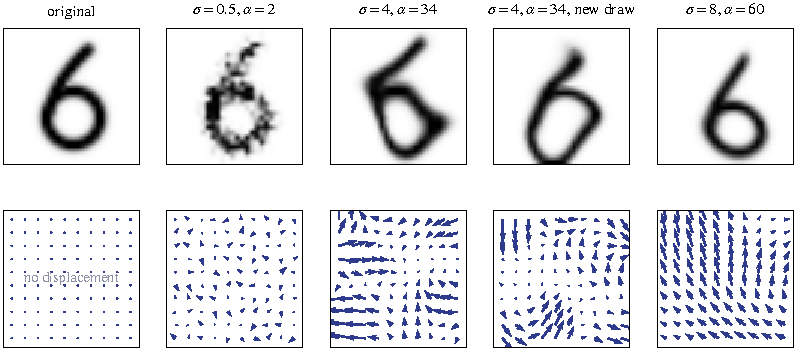
\includegraphics[width=\linewidth]{figures/n13_elastic.pdf}
\caption{Elastic distortions of a synthetic $28 \times 28$ digit (top) and the displacement fields that produced them
(bottom, every third pixel, arrows drawn to scale). With $\sigma = 0.5$ the field is nearly independent from pixel to pixel
and tears the stroke; with $\sigma = 4$ and $\alpha = 34$ it bends the digit coherently (root-mean-square displacement
$2.6$ pixels in the first draw); two draws give two different, plausible sixes. With $\sigma = 8$ the field is nearly
uniform over the image.}
\label{fig:elastic}
\end{figure}

\begin{algorithm}[htbp]
\caption{Elastic distortion of an image}\label{alg:elastic}
\begin{algorithmic}[1]
\Require image $x \in \R^{H \times W}$ (one channel; apply the same field to every channel); width $\sigma$; intensity $\alpha$
\Function{ElasticDistort}{$x$; $\sigma, \alpha$}
  \State draw $\Delta u_{u,v}, \Delta v_{u,v} \sim \mathrm{Uniform}[-1, 1]$ independently for every pixel
  \State $\Delta u \gets \alpha\, (G_\sigma * \Delta u)$; \ $\Delta v \gets \alpha\, (G_\sigma * \Delta v)$
    \Comment{Gaussian smoothing, separable, $O(HW\sigma)$}
  \For{every pixel $(u, v)$}
    \State $x'_{u,v} \gets \textsc{Bilinear}(x;\ u + \Delta u_{u,v},\ v + \Delta v_{u,v})$
      \Comment{weighted mean of four neighbours}
  \EndFor
  \State \Return $x'$ \Comment{called anew each time an image enters a mini-batch}
\EndFunction
\end{algorithmic}
\end{algorithm}

\begin{runtime}{elastic distortion and on-the-fly augmentation}
\emph{Time}: $O(HW\sigma)$ per image for the separable smoothing (two one-dimensional Gaussian filters of length
$\approx 6\sigma$ per field component) and $O(HW)$ for the interpolation --- small compared with a forward pass through the
network, and it can run on the CPU while the GPU trains. \emph{Memory}: $O(HW)$ for the field; augmenting on the fly stores
no extra examples, whereas precomputing $A$ transformed copies of $n$ images would need $A$ times the storage.
\emph{Training time} per epoch is unchanged, though more epochs are usually needed.
\emph{Prediction}: no cost, unless predictions are averaged over several augmented copies of the test image (test-time
augmentation), which multiplies the prediction cost by the number of copies.
\end{runtime}

\begin{modern}{augmentation in current practice}
The standard ImageNet recipe since AlexNet uses random crops and horizontal flips; modern pipelines add random
resizing, colour jitter and policies chosen automatically. \emph{Mixup}~\cite{zhang2018} goes beyond label-preserving
transformations: it trains on convex combinations $\lambda\x_i + (1 - \lambda)\x_j$ of two inputs with the same
combination of their one-hot labels. In self-supervised learning augmentation even defines the task: SimCLR~\cite{chen2020}
trains a network to map two random augmentations of the same image to nearby representations and those of different
images far apart, with no labels at all. The choice of augmentations then determines which invariances the representation
acquires.
\end{modern}

\begin{physics}{jet images: augment or standardise}
At the Large Hadron Collider the energy deposits of a jet in the calorimeter can be drawn as an image on the
(pseudorapidity, azimuth) plane, with pixel intensities equal to the transverse energy. Cogan et al.\ introduced such
jet images~\cite{cogan2015}, and convnets trained on them separate jets from boosted $W$ bosons from ordinary quark and
gluon jets~\cite{deoliveira2016}. Some symmetries are
exact here --- a shift in azimuth, a rotation about the jet axis to good approximation --- and there are two ways to use
them. One can augment, showing the network randomly rotated and translated copies; or one can remove the nuisance
variation by preprocessing, centring every jet on its leading subjet and rotating it into a standard orientation, as these
studies do. Preprocessing is cheaper and exact when the symmetry is; augmentation is the only option when no canonical
orientation exists; equivariant architectures (Section~\ref{sec:equiv}) are a third option.
\end{physics}

\section{From AlexNet to residual networks}\label{sec:history}

\paragraph{AlexNet} The ImageNet Large Scale Visual Recognition Challenge (ILSVRC) asks for one of 1000 classes for each
image and provides about 1.2~million labelled training images~\cite{deng2009}. In 2012 Krizhevsky, Sutskever and Hinton
entered a convnet with five convolutional and three fully connected layers, 60~million parameters and 650\,000
neurons~\cite{krizhevsky2012} (the timeline of Note~11, Section~8, places it in context). Trained on two GPUs for about a week, it reached a top-5 test error of $15.3\%$ (the true
class is not among the five highest-scoring guesses), against $26.2\%$ for the best entry built on hand-designed
features. Its ingredients were few and are all standard now: ReLU activations, which trained several times faster than
saturating units (and variants followed, such as maxout units, the maximum of several linear
functions~\cite{goodfellow2013}); dropout in the fully connected layers (Note~12, Section~6.3); heavy data augmentation (Section~\ref{sec:augment}); and
a fast GPU implementation of convolutions. The result ended the era of hand-designed visual features; within a few
years almost all entries were convnets.

\paragraph{What the filters learn} The first-layer filters of a trained convnet can be displayed directly as small
images. They are oriented edge detectors at various scales and frequencies, and colour-contrast blobs --- strikingly
similar to the receptive fields Hubel and Wiesel found, and to the Gabor filters designed by hand before. Deeper units are
not filters on pixels and must be visualised indirectly: by the training patches that excite them most, or by projecting
their activation back to pixel space. Zeiler and Fergus did the latter with a ``deconvolutional'' network built from the
transposed operations of Section~\ref{sec:transposed}~\cite{zeiler2014}. They found a hierarchy: corners and conjunctions of
edges in the second layer, textures and repeated patterns in the third, object parts such as dog faces and bird legs in
the fourth, and whole objects in varied poses in the fifth. The visualisations also diagnosed problems --- aliasing caused by the large first-layer stride --- and a
network with smaller first-layer filters and stride performed better.

\paragraph{Deeper, with small filters} VGG networks~\cite{simonyan2015} used only $3 \times 3$ convolutions, stacked
$16$ or $19$ weight layers deep, and showed that depth itself improves accuracy. GoogLeNet~\cite{szegedy2015} combined $1 \times 1$, $3 \times 3$ and
$5 \times 5$ convolutions in parallel ``inception'' modules.

\begin{worked}{8. Why small filters, and why bottlenecks}
\emph{Stacking.} Two $3 \times 3$ layers in a row see a $5 \times 5$ patch, by \eqref{eq:rf}: $1 + 2 + 2 = 5$. With $C$
channels in and out (biases ignored) they have $2 \times 9C^2 = 18C^2$ weights, against $25C^2$ for one $5 \times 5$ layer;
three $3 \times 3$ layers see $7 \times 7$ with $27C^2$ weights against $49C^2$. For $C = 256$: $1\,179\,648$ against
$1\,638\,400$, and $1\,769\,472$ against $3\,211\,264$. The stack also inserts a non-linearity between the layers, so it is
cheaper \emph{and} more expressive.

\emph{Bottleneck.} A residual block of the deeper ResNets (below) acting on 256 channels uses $1 \times 1$ convolutions to go
down to 64 channels, a $3 \times 3$ convolution at 64 channels, and a $1 \times 1$ convolution back up to 256:
\[
  256 \cdot 64 + 9 \cdot 64 \cdot 64 + 64 \cdot 256 = 16\,384 + 36\,864 + 16\,384 = 69\,632
\]
weights, against $2 \times 9 \times 256^2 = 1\,179\,648$ for two $3 \times 3$ convolutions at 256 channels --- seventeen times
fewer, at the same input and output width.
\end{worked}

\paragraph{Residual networks} Making plain convnets deeper eventually made them \emph{worse}, on the training set as well
as on the test set, which is an optimisation problem, not overfitting. In the residual networks of He, Zhang, Ren and
Sun~\cite{he2016} each block adds a learned correction to its input,
\begin{equation}\label{eq:resblock}
  \vect{h}_{\mathrm{out}} = \ReLU\big(\vect{h} + F(\vect{h})\big),
\end{equation}
where $F$ is two or three convolutions with batch normalisation (Note~12, Section~10.2) and ReLUs in between; why this
keeps very deep stacks trainable is derived in Note~12, Section~10.3. Two details are specific to convnets. When $F$
changes the number of channels or uses stride 2, the shortcut becomes a $1 \times 1$ convolution with the same stride, so
that the shapes match. And the original block applies the ReLU \emph{after} the addition, unlike the pre-normalised
form of Note~12, Section~10.3. With this design networks of 152 layers trained well, and an ensemble of them won ILSVRC~2015 with a
top-5 error of $3.57\%$; an often-quoted estimate of trained human top-5 error on the same task is about
$5\%$~\cite{russakovsky2015}.

\begin{algorithm}[htbp]
\caption{Residual block of a convnet (basic form)}\label{alg:res}
\begin{algorithmic}[1]
\Require feature maps $h \in \R^{C \times H \times W}$; two $3 \times 3$ convolutions with $C'$ output channels, the first
  with stride $s$; normalisation layers $N_1, N_2$
\Function{ResidualBlock}{$h$}
  \State $u \gets \ReLU\big(N_1(\textsc{Conv}_{3\times3,\,s}(h))\big)$ \Comment{Algorithm~\ref{alg:conv}, padding 1}
  \State $u \gets N_2(\textsc{Conv}_{3\times3,\,1}(u))$
  \If{$C' \ne C$ or $s \ne 1$}
    \State $h \gets \textsc{Conv}_{1\times1,\,s}(h)$ \Comment{projection shortcut, matches the shape of $u$}
  \EndIf
  \State \Return $\ReLU(h + u)$ \Comment{add, then activate}
\EndFunction
\end{algorithmic}
\end{algorithm}

\begin{runtime}{residual block}
\emph{Time}: two $3 \times 3$ convolutions, $9C'(C + C')\Hout\Wout$ multiply--adds per example, plus $CC'\Hout\Wout$ for a
projection shortcut and $O(C'\Hout\Wout)$ for the addition, normalisations and activations. The identity shortcut is
free. \emph{Memory}: $9C'(C + C')$ weights (plus $CC'$ for a projection); activations of both convolutions are stored for
the backward pass. \emph{Backward}: about twice the forward cost; the shortcut adds no cost (Note~12, Section~10.3).
\end{runtime}

\paragraph{Attention to channels} Squeeze-and-excitation blocks~\cite{hu2018} add a cheap form of global context: average
each of the $C$ channels over all positions to a vector $\vect{s} \in \R^C$, pass it through a small two-layer network
ending in a sigmoid to obtain channel weights $\vect{g} \in (0, 1)^C$, and multiply channel $c$ by $g_c$. With a
reduction from $C$ to $C/r$ hidden units this costs $2C^2/r$ weights: $8192$ for $C = 256$ and $r = 16$. An ensemble of
SE networks won the final ILSVRC, in 2017, with a top-5 error of $2.25\%$~\cite{hu2018}. Algorithm~\ref{alg:se} also
gives the \emph{depthwise separable} convolution of the box below, which factorises a $k \times k$ layer into a
per-channel spatial filter and a $1 \times 1$ channel mixer.

\begin{algorithm}[htbp]
\caption{Squeeze-and-excitation block and depthwise separable convolution}\label{alg:se}
\begin{algorithmic}[1]
\Require feature maps $h \in \R^{C \times H \times W}$; $W_1 \in \R^{(C/r) \times C}$, $W_2 \in \R^{C \times (C/r)}$, biases
  $\vect{b}_1, \vect{b}_2$
\Function{SqueezeExcite}{$h$}
  \State $s_c \gets \frac{1}{HW}\sum_{u,v} h_{c,u,v}$ for each $c$ \Comment{squeeze: global average pooling}
  \State $\vect{g} \gets \operatorname{sigmoid}\big(W_2\,\ReLU(W_1\vect{s} + \vect{b}_1) + \vect{b}_2\big)$
    \Comment{excite: $C \to C/r \to C$}
  \State \Return $h'_{c,u,v} = g_c\, h_{c,u,v}$ \Comment{rescale each channel}
\EndFunction
\Function{DepthwiseSeparable}{$x$; $k \times k$ kernels $D_{c'}$, $1 \times 1$ weights $V \in \R^{\Cout \times \Cin}$}
  \State $q_{c'} \gets x_{c'} \star D_{c'}$ for each input channel $c'$ \Comment{depthwise: $\Cin k^2$ weights}
  \State \Return $z_{c,u,v} = \sum_{c'} V_{c,c'}\, q_{c',u,v}$ \Comment{pointwise: $\Cin\Cout$ weights}
\EndFunction
\end{algorithmic}
\end{algorithm}

\begin{runtime}{squeeze-and-excitation and depthwise separable convolution}
\emph{SE time}: $O(CHW)$ for the squeeze and for the rescaling (each entry is read once), $O(2C^2/r)$ for the two small
layers --- negligible next to the convolutions around it. \emph{SE memory}: $2C^2/r$ weights plus $C/r + C$ biases.
\emph{Depthwise separable time}: $O(\Cin\Hout\Wout k^2)$ for the per-channel filters plus $O(\Cin\Cout\Hout\Wout)$ for
the channel mixing, instead of $O(\Cin\Cout\Hout\Wout k^2)$: a saving of almost $k^2$ when $\Cout \gg k^2$.
\emph{Memory}: $\Cin(k^2 + 1) + \Cout(\Cin + 1)$ parameters with biases. \emph{Prediction}: the same as the forward pass.
\end{runtime}

\begin{modern}{patches, transformers and convnets today}
The vision transformer (ViT)~\cite{dosovitskiy2021} cuts a $224 \times 224$ image into $16 \times 16$ patches and maps
each to a vector of dimension $D$ by one shared linear map. That patch embedding \emph{is} a convolution with kernel size
$16$ and stride $16$: by Worked example~10 it produces a $14 \times 14 = 196$-position
map with $D$ channels, and for $D = 768$ it has $16 \cdot 16 \cdot 3 \cdot 768 + 768 = 590\,592$ parameters. Everything
after it is a transformer: attention (Note~5, Section~3.3) lets every patch interact with every other from the first layer on, and locality
survives only in the patch embedding. Without this prior ViT needs more data: trained on ImageNet alone it falls behind
comparable ResNets, while pre-trained on far larger data sets it matches or surpasses them. ConvNeXt~\cite{liu2022} then
modernised the ResNet with large $7 \times 7$ depthwise convolutions (the separable design of
MobileNets~\cite{howard2017}, Algorithm~\ref{alg:se}), layer normalisation (Note~12, Section~10.2) and GELU (Note~11,
Section~2), and competes with vision transformers. Locality and sharing remain good priors; how much of them to hard-wire depends on
how much data is available.
\end{modern}

\section{Convolution arithmetic}\label{sec:arith}

This section collects the bookkeeping that every practical convnet needs: the matrix form of a convolution, the size of
its output, padding, stride and dilation, and inputs of variable size. We follow the conventions of Dumoulin and
Visin~\cite{dumoulin2016}: along one spatial axis, $i$ is the input size, $k$ the kernel size, $s$ the stride, the step
by which the window advances, $p$ the number of zeros appended on \emph{both} sides of the axis, and $o$ the output
size. Axes are treated independently, so non-square images and kernels
need nothing new.

\subsection{Convolution is a sparse matrix product}\label{sec:matrix}

Unroll the input into a vector (rows one after the other) and the output likewise. A convolution is linear in its input,
so $\y = C\x$ for some matrix $C$. Row $j$ of $C$ holds the kernel at the positions of window $j$ and zeros elsewhere.

\begin{worked}{9. A convolution written as a matrix}
\emph{One dimension.} The convolution of Worked example~2, $i = 5$, $k = 3$, $s = 1$ and $w = (1, 0, -1)$, reads
\[
  \begin{pmatrix} y_0 \\ y_1 \\ y_2 \end{pmatrix} =
  \begin{pmatrix} 1 & 0 & -1 & 0 & 0 \\ 0 & 1 & 0 & -1 & 0 \\ 0 & 0 & 1 & 0 & -1 \end{pmatrix}
  \begin{pmatrix} x_0 \\ x_1 \\ x_2 \\ x_3 \\ x_4 \end{pmatrix},
\]
and with $x = (2, 3, 5, 4, 1)$ it returns $(-3, -1, 4)$, as before. Each row is the previous one shifted right by $s$ (a
\emph{Toeplitz} structure, constant along diagonals). With stride $2$ only every second row would be kept.

\emph{Two dimensions.} For a $5 \times 5$ input and a $3 \times 3$ kernel, $C$ is $9 \times 25$: each of the nine rows
contains the nine kernel entries, arranged in three groups of three separated by two zeros (the jump to the next image
row), and zeros elsewhere --- $81$ non-zeros out of $225$ entries, or $36\%$. Here $C$ is fairly dense only because the image is tiny.
For a $224 \times 224$ image, a $3 \times 3$ kernel and an output of the same size, $C$ is $50\,176 \times 50\,176$ with
at most $9$ non-zeros per row, a fraction $9/50\,176 \approx 1.8 \times 10^{-4}$ of its entries, and only $9$
distinct values.
\end{worked}

The matrix view explains two facts at once. First, a convolutional layer is a fully connected layer whose weight matrix
is constrained to be sparse (local connectivity) and to repeat the same values (sharing); everything known about MLPs
applies. Second, by the chain rule $\partial \ell/\partial\x = C\T\,\partial \ell/\partial\y$: the backward pass multiplies by the
\emph{transpose}. Equation~\eqref{eq:gradx} is exactly multiplication by $C\T$; Section~\ref{sec:transposed} uses $C\T$
as a layer in its own right.

\paragraph{The im2col form} Libraries rarely loop as in Algorithm~\ref{alg:conv}. They copy every receptive field, a
$\Cin k^2$ vector, into one row of a \emph{patch matrix} $P$ with $\Hout\Wout$ rows (``image to columns''), and compute
all outputs with a single dense matrix product $P\,\tilde W\T$, where $\tilde W \in \R^{\Cout \times \Cin k^2}$ holds one
flattened filter per row. Dense matrix products run close to the peak speed of GPUs, which more than pays for the
copying.

\begin{algorithm}[htbp]
\caption{Convolution as one matrix product (im2col)}\label{alg:im2col}
\begin{algorithmic}[1]
\Require padded input $\bar x \in \R^{\Cin \times (H + 2p) \times (W + 2p)}$; weights $W$; biases $\vect{b}$; stride $s$
\Function{Im2colConv}{$\bar x$; $W, \vect{b}, s$}
  \State $P \gets$ empty matrix with $\Hout\Wout$ rows and $\Cin k^2$ columns
  \For{$u = 0, \dots, \Hout - 1$; \ $v = 0, \dots, \Wout - 1$}
    \State row $(u\Wout + v)$ of $P$ $\gets$ $\bar x_{\cdot,\ su:su+k,\ sv:sv+k}$ flattened \Comment{copy, no arithmetic}
  \EndFor
  \State $\tilde W \gets W$ reshaped to $\Cout \times \Cin k^2$
  \State $Z \gets P\,\tilde W\T + \vect{1}\vect{b}\T$ \Comment{one GEMM, $\Hout\Wout \times \Cout$}
  \State \Return $Z$ reshaped to $\Cout \times \Hout \times \Wout$
\EndFunction
\end{algorithmic}
\end{algorithm}

\needspace{9\baselineskip}
\begin{runtime}{im2col convolution}
\emph{Time}: $O(\Hout\Wout\Cin k^2)$ to build $P$ and $O(\Hout\Wout\Cin k^2\Cout)$ for the product, the same multiply--add
count as the direct form but executed as one highly optimised matrix multiplication. \emph{Memory}: $P$ duplicates every
input value up to $k^2$ times: for $64$ channels on a $56 \times 56$ map with $k = 3$ it holds $1.8 \times 10^6$ numbers
($7.2$~MB in 32-bit floats) against $0.2 \times 10^6$ for the map itself. Alternatives trade differently: FFT-based
convolution costs $O(HW\log(HW))$ per pair of channels and pays off for large kernels, and specialised small-kernel
algorithms reduce the multiplication count further for $3 \times 3$ filters.
\end{runtime}

\subsection{Output size, padding and stride}

\paragraph{Derivation of the output size} After padding, the axis has $i + 2p$ entries, numbered $0, \dots, i + 2p - 1$.
The kernel starts at positions $0, s, 2s, \dots$; a start $js$ is allowed if the window ends inside the axis,
$js + k - 1 \le i + 2p - 1$, that is $j \le (i + 2p - k)/s$. Counting $j = 0, 1, \dots$ up to the largest such integer gives
\begin{equation}\label{eq:osize}
  o = \left\lfloor \frac{i + 2p - k}{s} \right\rfloor + 1 .
\end{equation}
When $s$ does not divide $i + 2p - k$, the last $(i + 2p - k) \bmod s$ positions of the padded axis lie in no window
and are ignored. For example $i = 7$ and $i = 8$ both give $o = 4$ with $k = 3$, $s = 2$, $p = 1$; and with $p = 0$ the
entry $x_7$ of a length-$8$ signal is never used ($o = 3$).

\paragraph{Three kinds of padding} Without padding the output shrinks by $k - 1$ in each layer, and border pixels take
part in fewer windows than central ones. Three choices are common for $s = 1$ (Figure~\ref{fig:padding}):
\begin{itemize}
\item \emph{valid} ($p = 0$): only complete windows, $o = i - k + 1$;
\item \emph{same} or \emph{half} ($p = (k - 1)/2$ for odd $k$): $o = i$, so that layers can be stacked without shrinking
  --- the usual choice, as in the $3 \times 3$, padding-1 layers of VGG and ResNet;
\item \emph{full} ($p = k - 1$): every window that overlaps the input in at least one entry, $o = i + k - 1$. This is the
  length of the full convolution of \eqref{eq:gradx}, and of the product of two polynomials of degrees $i - 1$ and $k - 1$.
\end{itemize}
Zero padding is the default. \emph{Reflect} padding (mirror the border) and \emph{circular} padding (wrap around) are
alternatives; the latter is the natural choice for periodic data.

\begin{figure}[htbp]
\centering
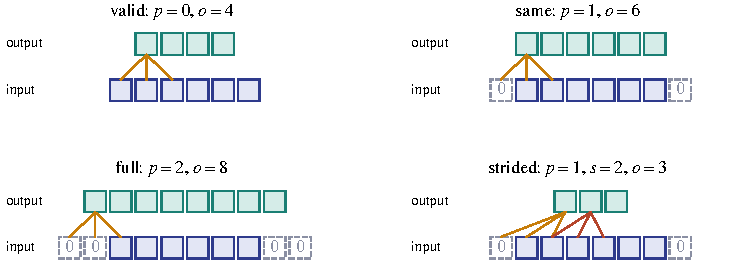
\includegraphics[width=0.9\linewidth]{figures/n13_padding.pdf}
\caption{Padding and stride along one axis for $i = 6$ and $k = 3$; dashed cells are the padding zeros. The lines show the
window of the first output (and, for stride $2$, of the second). Valid, same and full padding give $o = 4, 6, 8$; with
$p = 1$ and $s = 2$, $o = \lfloor 5/2 \rfloor + 1 = 3$.}
\label{fig:padding}
\end{figure}

\needspace{16\baselineskip}
\begin{worked}{10. Output sizes}
By \eqref{eq:osize}, with the arguments $(i, k, s, p)$ (and $k$ replaced by $\hat k$ of \eqref{eq:kdil} for a dilation
$d > 1$):
\begin{center}\small
\begin{tabular}{@{}lll@{}}
\toprule
$(i, k, s, p)$ & computation & $o$ \\
\midrule
$(6, 3, 1, 0)$ & $\lfloor 3/1 \rfloor + 1$ & $4$ \\
$(6, 3, 1, 1)$, same & $\lfloor 5/1 \rfloor + 1$ & $6$ \\
$(6, 4, 1, 2)$, even kernel & $\lfloor 6/1 \rfloor + 1$ & $7$ \\
$(7, 3, 2, 1)$ & $\lfloor 6/2 \rfloor + 1$ & $4$ \\
$(7, 3, 2, 0)$ & $\lfloor 4/2 \rfloor + 1$ & $3$ \\
$(10, 3, 1, 0)$, $d = 3$, $\hat k = 7$ & $\lfloor 3/1 \rfloor + 1$ & $4$ \\
$(32, 3, 1, 2)$, $d = 2$, $\hat k = 5$, same & $\lfloor 31/1 \rfloor + 1$ & $32$ \\
$(224, 7, 2, 3)$, first layer of a ResNet & $\lfloor 223/2 \rfloor + 1$ & $112$ \\
$(227, 11, 4, 0)$, AlexNet-like first layer & $\lfloor 216/4 \rfloor + 1$ & $55$ \\
$(224, 16, 16, 0)$, ViT patches & $\lfloor 208/16 \rfloor + 1$ & $14$ \\
\bottomrule
\end{tabular}
\end{center}
An even kernel cannot be centred, so ``same'' padding with $k = 4$ needs unequal padding on the two sides ($1$ and $2$);
$p = 2$ on both sides gives one extra output. Pooling obeys the same formula: $2 \times 2$ pooling with stride $2$ on a
$28$-pixel axis gives $\lfloor 26/2 \rfloor + 1 = 14$.
\end{worked}

\subsection{Dilation}

A \emph{dilated} (or atrous) convolution spreads the $k$ kernel entries out, with $d - 1$ skipped positions between
consecutive entries:
\[
  y_j = \sum_{m=0}^{k-1} w_m\, x_{j + d\,m} .
\]
The dilation $d = 1$ is an ordinary convolution. The kernel still has $k$ weights but spans
\begin{equation}\label{eq:kdil}
  \hat k = k + (k - 1)(d - 1)
\end{equation}
input positions, and the output size is \eqref{eq:osize} with $k$ replaced by $\hat k$ (two rows of the table of Worked
example~10). Dilation enlarges the receptive field without extra weights, without extra
computation and without the loss of resolution that pooling or strides cause; it is used for dense prediction tasks such
as segmentation~\cite{yu2016} and, with exponentially growing $d$, in the audio models of Section~\ref{sec:dilated}.

\subsection{Inputs of variable size}

Convolutions and pooling accept any input size; only their output size changes. The fully connected layers at the end of
LeNet or AlexNet do not: they need a fixed number of inputs. Two remedies are common. Pooling regions can be made
proportional to the input, so that the pooled map always has the same size. More simply, \emph{global average pooling}
averages each of the last $C$ feature maps over all its positions and passes the resulting $C$-vector to the classifier,
whatever the image size~\cite{lin2014}; it also removes the parameter-heavy fully connected layers (compare the table of
Worked example~6). A network made only of convolutions, pooling and pointwise operations is called \emph{fully
convolutional}; it maps an image of any size to a map of outputs, which Section~\ref{sec:transposed} exploits.

\begin{physics}{periodic lattices and circular padding}
Monte Carlo configurations of a lattice model, such as the two-dimensional Ising model on an $L \times L$ lattice with
periodic boundary conditions, are natural inputs for a convnet: the Hamiltonian is local and translation invariant, which
are exactly the assumptions of Section~\ref{sec:sharing}. Carrasquilla and Melko showed that neural networks trained on
such configurations can classify the ordered and disordered phases and locate the transition~\cite{carrasquilla2017}.
With periodic boundaries there is no edge, so zero padding would invent one; with stride-1 layers and no intermediate
pooling, circular padding makes every layer exactly equivariant under lattice translations, and a final global average
pool makes the prediction exactly invariant (with strides or pooling, only under shifts by multiples of the total
stride). A network
built this way can be trained on small lattices and applied, unchanged, to larger ones --- a useful check of finite-size
scaling.
\end{physics}

\section{Causal dilated stacks: WaveNet and ByteNet}\label{sec:dilated}

Raw audio has structure on many time scales at once: individual oscillations last a fraction of a millisecond, phonemes
tens of milliseconds, words and notes much longer. WaveNet~\cite{vandenoord2016} generates audio one sample at a time, at
$16\,000$ samples per second, predicting each sample from the samples before it. Two kinds of one-dimensional
convolution make this possible.

\paragraph{Causal convolutions} For generation the output at time $t$ may depend only on inputs at times $\le t$. A
\emph{causal} convolution achieves this by padding only on the left, with $\hat k - 1$ zeros: the output keeps the
length of the input and $y_t$ depends on $x_{t - \hat k + 1}, \dots, x_t$.

\paragraph{Exponentially dilated stacks} With kernel size $k = 2$ and dilations $1, 2, 4, \dots, 2^{L-1}$ in successive layers,
each layer adds $d_l(k - 1)$ to the receptive field, so by \eqref{eq:rf} (strides $1$, kernels of span $\hat k_l = d_l + 1$)
\[
  r = 1 + \sum_{l=1}^{L} d_l = 1 + (1 + 2 + \dots + 2^{L-1}) = 2^L .
\]
The receptive field doubles with every layer, while the number of weights and the cost grow only linearly in $L$
(Figure~\ref{fig:dilated}).

\begin{figure}[htbp]
\centering
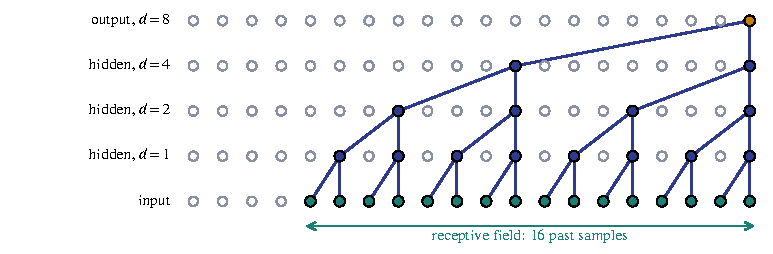
\includegraphics[width=0.95\linewidth]{figures/n13_dilated.pdf}
\caption{A stack of causal convolutions with kernel size $2$ and dilations $1, 2, 4, 8$. The highlighted connections feed
the last output; it depends on exactly the $2^4 = 16$ most recent inputs, with $4$ layers of $2$ weights each.}
\label{fig:dilated}
\end{figure}

\needspace{7\baselineskip}
\begin{worked}{11. Receptive fields of WaveNet}
WaveNet stacks blocks with dilations $1, 2, 4, \dots, 512$ ($L = 10$ layers, $k = 2$). One block has receptive field
$2^{10} = 1024$ samples, $64$~ms at $16$~kHz. Repeating the block three times adds $1023$ samples per block:
$1 + 3 \times 1023 = 3070$ samples, about $0.19$~s. Reaching $1024$ samples with undilated $k = 2$ convolutions would take
$1023$ layers; with $k = 3$ undilated, $512$ layers.
\end{worked}

The audio model also uses gated activations $\tanh(\cdot) \odot \sigma(\cdot)$, residual and skip connections, and a
softmax over $256$ quantised amplitude levels for each sample --- classification, sample by sample. The same causal
dilated stacks were used for machine translation (ByteNet~\cite{kalchbrenner2016}), before transformers took over that
role.

\begin{algorithm}[htbp]
\caption{Stack of dilated causal convolutions (one channel per layer for clarity)}\label{alg:dilated}
\begin{algorithmic}[1]
\Require sequence $x_0, \dots, x_{T-1}$; layers $l = 1, \dots, L$ with weights $w^{(l)} \in \R^k$, bias $b^{(l)}$,
  dilation $d_l$; activation $g$
\Function{DilatedCausalStack}{$x$}
  \State $h^{(0)} \gets x$
  \For{$l = 1, \dots, L$}
    \For{$t = 0, \dots, T - 1$}
      \State $h^{(l)}_t \gets g\big(b^{(l)} + \sum_{m=0}^{k-1} w^{(l)}_m\, h^{(l-1)}_{t - d_l(k - 1 - m)}\big)$
        \Comment{$h_{t'} = 0$ for $t' < 0$: left padding}
    \EndFor
  \EndFor
  \State \Return $h^{(L)}$ \Comment{depends on $x_{t - r + 1}, \dots, x_t$ only, $r = 1 + (k - 1)\sum_l d_l$}
\EndFunction
\end{algorithmic}
\end{algorithm}

\begin{runtime}{dilated causal stack}
\emph{Time}: $O(TLkC^2)$ for $T$ time steps, $L$ layers and $C$ channels per layer, the same as undilated convolutions;
the receptive field $1 + (k - 1)\sum_l d_l$ grows exponentially in $L$ for $d_l = 2^{l-1}$. \emph{Training} is parallel
over all $T$ positions because the whole target sequence is known. \emph{Generation} is sequential: each new sample needs a
pass through all $L$ layers, $O(LkC^2)$ per sample if the past activations of every layer are cached (otherwise
$O(rLkC^2)$), and $16\,000$ such passes per second of audio. \emph{Memory}: $LkC^2$ weights; the cache needs
$(k - 1)d_l$ past values per layer and channel.
\end{runtime}

\begin{physics}{one-dimensional convnets on detector time series}
Many physics signals are long one-dimensional series in which a short, characteristic pattern must be found anywhere:
a gravitational-wave chirp in interferometer strain data, a pulse in a photomultiplier trace, a transit in a stellar light
curve. Translation equivariance in time is the right prior, and the receptive field must cover the longest pattern. George and
Huerta trained one-dimensional convnets directly on simulated detector strain to detect binary black-hole mergers and
estimate their parameters~\cite{george2018}, an alternative to matched filtering against a bank of templates that is far
cheaper at prediction time.
\end{physics}

\section{Structured outputs: transposed convolutions and upsampling}\label{sec:transposed}

In \emph{semantic segmentation} every pixel receives a class label (road, car, pedestrian; tumour or healthy tissue); in
image generation, super-resolution or the prediction of a physical field, the output is itself an image. A fully
convolutional network~\cite{long2015} can produce such outputs: an \emph{encoder} of convolutions and pooling reduces the
image to a small, deep feature map, and a \emph{decoder} enlarges it back to the input resolution, ending in a per-pixel
softmax or regression. The decoder needs a layer that \emph{increases} spatial size.

A parameter-free option is \emph{max-unpooling}~\cite{zeiler2014}: the decoder puts each value at the position recorded
by the matching encoder's max-pooling layer (the indices $\mathrm{arg}$ of Algorithm~\ref{alg:pool}) and fills the rest of
the block with zeros, exactly what \textsc{MaxPoolBackward} does with a gradient. It restores \emph{where} features
were, not what surrounded them, and is followed by convolutions. Two learnable layers are in use as well.

\subsection{Transposed convolution}

A convolution maps $\x \in \R^i$ to $\y = C\x \in \R^o$, with $o \le i$ for the usual choices $p \le (k - 1)/2$. The
\emph{transposed convolution} uses the same sparse structure in the other direction, $\x' = C\T\y'$: from $o$ values to $i$.
Read column by column, $C\T\y' = \sum_j y'_j\,(\text{row } j \text{ of } C)\T$: each input value $y'_j$ \emph{scatters} a
scaled copy of the kernel onto the output, at position $js$, and overlapping copies add. As Section~\ref{sec:matrix}
showed, this is the backward pass of a convolution, now used in the forward direction with learned weights. It is not an
inverse: $C\T C \ne I$ in general. The name ``deconvolution'' is common but misleading; ``fractionally strided
convolution'' describes an equivalent implementation: insert $s - 1$ zeros between consecutive input values, pad with
$k - 1 - p$ zeros on each side, and cross-correlate with the flipped kernel at stride $1$ --- equivalent, but wasteful,
since most multiplications are by zero.

The output size inverts \eqref{eq:osize}. If $s$ divides $i + 2p - k$, \eqref{eq:osize} reads $o - 1 = (i + 2p - k)/s$;
solving for $i$, a transposed convolution with parameters $(k, s, p)$ maps $o$ entries to
\begin{equation}\label{eq:tsize}
  i' = s(o - 1) + k - 2p ,
\end{equation}
the input size of the corresponding convolution when $s$ divides $i + 2p - k$. Otherwise several input sizes share the
same $o$ (Section~\ref{sec:arith}), and libraries take an extra ``output padding'' argument to choose among them.

\begin{worked}{12. A transposed convolution by hand, and its checkerboard}
\emph{Scatter.} Input $\y' = (1, 2, -1)$, kernel $w = (1, 2, 1)$, stride $2$, no padding. By \eqref{eq:tsize} the output
has $2 \cdot 2 + 3 = 7$ entries. Each input value places a scaled kernel, two positions further along each time:
\[
  (1, 2, 1, 0, 0, 0, 0) + (0, 0, 2, 4, 2, 0, 0) + (0, 0, 0, 0, -1, -2, -1) = (1, 2, 3, 4, 1, -2, -1) .
\]
\emph{Check with the matrix.} The convolution with $i = 7$, $k = 3$, $s = 2$ has $o = 3$ and
\[
  C = \begin{pmatrix} 1 & 2 & 1 & 0 & 0 & 0 & 0 \\ 0 & 0 & 1 & 2 & 1 & 0 & 0 \\ 0 & 0 & 0 & 0 & 1 & 2 & 1 \end{pmatrix},
  \qquad C\T(1, 2, -1)\T = (1, 2, 3, 4, 1, -2, -1)\T .
\]
\emph{Check with zero insertion.} $(1, 2, -1)$ becomes $(1, 0, 2, 0, -1)$, padded with $k - 1 - p = 2$ zeros on each side;
cross-correlating with the flipped kernel, here again $(1, 2, 1)$, gives the same seven numbers, with only $9$ of the
$21$ products non-zero.

\emph{Uneven overlap.} Feed a constant input $(1, 1, 1, 1)$ and the kernel $(1, 1, 1)$ with stride $2$. The output is
$(1, 1, 2, 1, 2, 1, 2, 1, 1)$: positions reached by two copies of the kernel get $2$, the others $1$, although the input
has no structure at all. With $k = 4$ and $s = 2$ the copies overlap evenly, and the interior of the output is constant,
$(\dots, 2, 2, 2, \dots)$. In two dimensions the pattern of a $k = 3$, $s = 2$ layer is the product of two such
alternations, with interior values $1$, $2$ and $4$: a checkerboard (Figure~\ref{fig:checker}).
\end{worked}

\begin{algorithm}[htbp]
\caption{Transposed convolution (one input and one output channel)}\label{alg:tconv}
\begin{algorithmic}[1]
\Require input $y' \in \R^{o_1 \times o_2}$; kernel $w \in \R^{k \times k}$; stride $s$; padding $p$
\Function{TransposedConv}{$y'$; $w, s, p$}
  \State $\bar x \gets$ zero array of size $(s(o_1 - 1) + k) \times (s(o_2 - 1) + k)$
  \For{$u = 0, \dots, o_1 - 1$; \ $v = 0, \dots, o_2 - 1$}
    \State $\bar x_{su:su+k,\ sv:sv+k} \mathrel{+}= y'_{u,v}\, w$ \Comment{scatter a scaled kernel; overlaps add}
  \EndFor
  \State \Return $\bar x$ without $p$ rows and columns on each side \Comment{size $s(o - 1) + k - 2p$ per axis}
\EndFunction
\end{algorithmic}
\end{algorithm}

\begin{runtime}{transposed convolution}
\emph{Time}: $O(o_1o_2k^2)$ per channel pair, so $O(\Cin\Cout o_1o_2k^2)$ for a layer --- the cost of the convolution it
transposes; the zero-insertion implementation wastes a factor of about $s^2$. \emph{Memory}: $\Cout(\Cin k^2 + 1)$
parameters, as for a convolution; the output is about $s^2$ times larger than the input, which dominates memory in the
high-resolution layers of a decoder. \emph{Backward}: the gradient of a transposed convolution is an ordinary
convolution, with the same cost.
\end{runtime}

\subsection{Checkerboard artefacts and resize-convolution}

When the kernel size is not divisible by the stride, the copies of the kernel overlap unevenly, and unless the weights
happen to compensate --- as the linear-interpolation kernel $(\tfrac12, 1, \tfrac12)$ with $s = 2$ does --- outputs carry
a periodic pattern even for perfectly smooth inputs (Worked example~12). A network can learn weights that cancel the pattern,
but in practice it often does not quite, and images generated by such decoders show faint checkerboards. Odena, Dumoulin
and Olah~\cite{odena2016} recommended two remedies: choose $k$ divisible by $s$ (for instance $k = 4$, $s = 2$), or
separate the two jobs --- first \emph{upsample} with a fixed interpolation (nearest neighbour or bilinear), then apply an
ordinary stride-1 convolution. The second, \emph{resize-convolution} (Algorithm~\ref{alg:resize}), cannot produce an
uneven overlap by construction and is now the usual choice in convolutional decoders that generate images
(Figure~\ref{fig:checker}).

\begin{algorithm}[htbp]
\caption{Resize-convolution (upsample by $s$, then convolve)}\label{alg:resize}
\begin{algorithmic}[1]
\Require $y' \in \R^{\Cin \times o_1 \times o_2}$; factor $s$; output $\Cout \times so_1 \times so_2$; weights $W \in \R^{\Cout \times \Cin \times k \times k}$ ($k$
  odd), biases $\vect{b}$
\Function{ResizeConv}{$y'$; $s, W, \vect{b}$}
  \State $u_{c,\,su+a,\,sv+b} \gets y'_{c,u,v}$ for all $0 \le a, b < s$ \Comment{nearest neighbour: copy into $s \times s$ blocks}
  \State \Return \Call{ConvForward}{$u$; $W, \vect{b}$, stride $1$, $p = (k - 1)/2$} \Comment{Algorithm~\ref{alg:conv}}
\EndFunction
\end{algorithmic}
\end{algorithm}

\begin{runtime}{resize-convolution}
\emph{Time}: $O(\Cin s^2o_1o_2)$ for the upsampling (one copy per fine-grid entry) plus $O(\Cout\Cin s^2o_1o_2k^2)$ for
the convolution, which now runs on the fine grid --- $s^2$ times the cost of a transposed convolution with the same $k$.
\emph{Memory}: $\Cout(\Cin k^2 + 1)$ parameters, as for any convolution, plus the upsampled intermediate
$\Cin s^2o_1o_2$, which is stored for the backward pass. \emph{Prediction}: the same as the forward pass.
\end{runtime}

\begin{figure}[htbp]
\centering
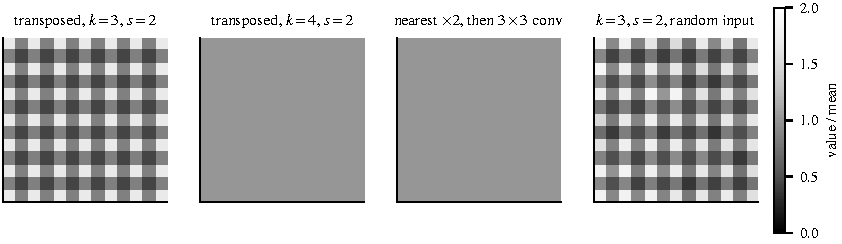
\includegraphics[width=\linewidth]{figures/n13_checkerboard.pdf}
\caption{Upsampling an $8 \times 8$ constant input by a factor $2$ (all kernel entries equal to one; borders cropped).
A transposed convolution with $k = 3$ and $s = 2$ produces a checkerboard with values $1$, $2$ and $4$; with $k = 4$ and
$s = 2$ the output is uniform, as it is with nearest-neighbour upsampling followed by a $3 \times 3$ convolution. Right:
the pattern of the $k = 3$ layer persists for a random input with values between $0.8$ and $1.2$.}
\label{fig:checker}
\end{figure}

\begin{modern}{U-Net, from microscopy to diffusion models}
Pooling discards precise positions, and a decoder alone cannot recover them. The U-Net of Ronneberger, Fischer and
Brox~\cite{ronneberger2015} adds \emph{skip connections}: the feature maps of each encoder level are concatenated with the
decoder maps of the same resolution, so that fine detail bypasses the bottleneck and coarse context comes up from below.
Designed for segmenting cells in microscope images from very few annotated examples --- with heavy elastic deformation as
augmentation (Section~\ref{sec:augment}) --- it became the standard image-to-image architecture. Denoising diffusion
models (Note~2, Section~5)~\cite{ho2020} use a U-Net to predict the noise added to an image, and latent diffusion
models~\cite{rombach2022} run such a U-Net on a compressed latent representation; many later systems replace it with a
transformer, but the encoder--decoder-with-skips idea remains.
\end{modern}

\begin{physics}{convolutional surrogates for field equations}
Many simulations produce fields on grids: velocity and pressure around a body, a density field in
cosmology. When the same kind of simulation must be run thousands of times, as in a design loop, an image-to-image network trained on a few thousand solved cases can act as a fast \emph{surrogate}.
Thuerey and co-workers trained U-Nets to predict the Reynolds-averaged velocity and pressure fields around airfoils from
the geometry and flow conditions, far faster than the solver~\cite{thuerey2020}. Local differential operators become local convolutions,
and the encoder's coarse levels carry the long-range part of the solution, like the coarse grids of a multigrid solver.
\end{physics}

\section{Costs at a glance}\label{sec:cost}

Table~\ref{tab:cost} collects the costs of this note for one example, with $\Cin$ and $\Cout$ channels, $k \times k$ kernels,
an input of $H \times W$ positions and an output of $\Hout \times \Wout$. Training costs about $3FnE$ for $F$ forward
multiply--adds (runtime box of Algorithm~\ref{alg:convback}).

\begin{table}[htbp]
\centering\small
\caption{Costs per example of the operations in this note (multiply--adds or comparisons).}
\label{tab:cost}
\begin{tabular}{@{}L{0.22\linewidth}L{0.24\linewidth}L{0.23\linewidth}L{0.22\linewidth}@{}}
\toprule
operation & forward time & parameters & stored for backward \\
\midrule
fully connected, $d \to m$ & $O(dm)$ & $m(d + 1)$ & $O(d + m)$ \\
convolution (direct or im2col) & $O(\Cout\Hout\Wout\Cin k^2)$ & $\Cout(\Cin k^2 + 1)$ & $O(\Cin HW + \Cout\Hout\Wout)$ \\
$1 \times 1$ convolution & $O(\Cout\Cin HW)$ & $\Cout(\Cin + 1)$ & $O((\Cin + \Cout)HW)$ \\
depthwise separable, $k \times k$ & $O(\Cin HW(k^2 + \Cout))$ & $\Cin(k^2 + 1) + \Cout(\Cin + 1)$ & $O((\Cin + \Cout)HW)$ \\
squeeze-and-excitation & $O(CHW + C^2/r)$ & $2C^2/r + C/r + C$ & $O(CHW)$ \\
max or average pooling & $O(CHW)$ & $0$ & $O(CHW/m^2)$ indices \\
dilated convolution & as convolution & as convolution & as convolution \\
max-unpooling & $O(CHW)$ & $0$ & --- \\
transposed convolution & $O(\Cout\Cin o_1o_2k^2)$ & $\Cout(\Cin k^2 + 1)$ & $O(\Cin o_1o_2)$ \\
resize-convolution, $\times s$ & $O(\Cout\Cin s^2o_1o_2k^2)$ & $\Cout(\Cin k^2 + 1)$ & $O(\Cin s^2o_1o_2)$ \\
residual block (basic) & $O(9C'(C + C')\Hout\Wout)$ & $9C'(C + C')$ & both convolutions \\
elastic distortion & $O(HW\sigma)$ & $0$ & --- \\
\bottomrule
\end{tabular}
\end{table}

\paragraph{Where the cost goes} Because each weight is reused at every position (Worked example~6), a convnet performs
many operations per parameter: it is \emph{compute-bound}, which is why GPUs mattered so much in 2012
(Section~\ref{sec:history}).

\begin{keyidea}[Summary]
Convolutional networks are MLPs with two constraints on the weights: each unit sees only a local patch of the input, and
all units of a feature map share the same weights. A layer computes cross-correlations of all input channels with a
$\Cin \times k \times k$ filter per output channel and has $\Cout(\Cin k^2 + 1)$ parameters, independently of the image
size. Convolution commutes with translations (equivariance); pooling summarises neighbourhoods and adds approximate local
invariance and subsampling. Other invariances are taught by data augmentation, including elastic distortions.
Backpropagation through a convolution sums the gradients of a shared weight over positions and sends the output gradient
back by the transposed operation, a full convolution. Stacks of small filters, $1 \times 1$ channel mixing and residual
blocks took convnets from AlexNet to networks hundreds of layers deep. The output size along an axis is
$\lfloor (i + 2p - k)/s \rfloor + 1$; dilation enlarges the effective kernel to $k + (k - 1)(d - 1)$ and gives
exponentially large receptive fields at linear cost; transposed convolutions and resize-convolutions enlarge feature maps
for segmentation and generation, and U-Nets combine both directions with skip connections.
\end{keyidea}

\needspace{12\baselineskip}
\begin{questions}
\begin{conceptual}
\item Name the three ideas that distinguish a convolutional layer from a fully connected one. For each, state the
  property of images it exploits and what it saves (parameters, computation, or data).
\item Explain why a convolutional layer can be seen as a fully connected layer with constraints on its weight matrix.
  Which entries are forced to be zero, and which are forced to be equal?
\item A convolutional layer with $3 \times 3$ kernels is applied to a $64 \times 64$ image and then to a $512 \times 512$
  image. Does the number of parameters change? Does the computation change? Explain.
\item Define translation \emph{equivariance} and translation \emph{invariance}. Which of the two does a convolutional layer
  have, which does max pooling approximately add, and which does a classifier ultimately need?
\item What is the difference between convolution and cross-correlation? Why does it not matter for a layer whose kernel
  is learned, and when does it matter?
\item A filter of the first layer of a network for colour images has size $3 \times 5 \times 5$. Explain what the three
  numbers mean and why the first one must equal the number of input channels.
\item Explain why max pooling gives only approximate invariance to translations. Describe a shift by one pixel that
  changes the output of $2 \times 2$ max pooling, and one that does not.
\item In a LeNet-style network most parameters are in the fully connected layers and most computation in the
  convolutional layers. Explain why.
\item How does the receptive field of a unit grow with depth in a stack of stride-1 $3 \times 3$ convolutions? What do
  pooling and dilation change?
\item Why does a convnet trained without augmentation not automatically recognise rotated digits? Give one
  transformation that is a sensible augmentation for photographs of animals but not for handwritten digits, and explain.
\item In an elastic distortion, what do the width $\sigma$ and the intensity $\alpha$ control? What goes wrong for very
  small $\sigma$?
\item Name the four ingredients that AlexNet combined, and say for each which section or note of this course explains it.
\item Why do two stacked $3 \times 3$ convolutions often replace one $5 \times 5$ convolution? Give two reasons.
\item What problem did residual connections solve in very deep convnets, and why was it an optimisation problem rather
  than overfitting? What must the shortcut do when a block changes the number of channels or uses stride 2?
\item Explain the role of a $1 \times 1$ convolution. Why is it called a fully connected layer applied at every pixel?
\item What does ``same'' padding achieve, and why is it awkward for even kernel sizes?
\item Explain how global average pooling allows a network to accept images of different sizes.
\item Jets in a calorimeter image can be handled by augmentation (random rotations) or by standardisation (rotating every
  jet into a fixed orientation). Give one advantage of each, and say when only augmentation is possible.
\item Why is a convolution of a $224 \times 224$ image best stored as a kernel and not as the matrix $C$ of
  Section~\ref{sec:matrix}? What does the matrix view nonetheless explain about the backward pass?
\item What is a causal convolution, and why does audio generation need it? Why is generation with WaveNet much slower
  than training?
\item Why is a transposed convolution not the inverse of a convolution? Explain where checkerboard artefacts come from
  and two ways to avoid them.
\item In a U-Net, what do the skip connections carry, and why can the decoder not recover this information on its own?
\item The patch embedding of a vision transformer is a convolution. With which kernel size and stride? Which prior of
  convnets does the rest of a transformer give up, and what is the price in terms of data?
\end{conceptual}

\begin{calculations}
\item Compute the cross-correlation and the convolution (valid, stride 1) of $x = (1, 3, 0, -2, 4)$ with
  $w = (2, -1)$. Then compute the cross-correlation with $w = (1, 1, 1)/3$ and describe what this kernel does.
\item Use the image $x$ and the kernel $w$ of Worked example~3. (a)~With zero padding $p = 1$ and stride $1$, compute the
  first row of the $4 \times 4$ output. (b)~With $p = 1$ and stride $2$, how large is the output? Compute its top-left
  entry. (c)~Apply $\ReLU$ to the $2 \times 2$ output of Worked example~3 with bias $0$ and then $2 \times 2$ max pooling.
\item Count the parameters and the forward multiply--adds of a convolutional layer with $\Cin = 32$, $\Cout = 64$,
  $k = 3$, stride $1$ and same padding on a $32 \times 32$ input (include the biases). Repeat for a depthwise separable layer (one $3 \times 3$
  filter per input channel, then a $1 \times 1$ convolution from 32 to 64 channels), and give the ratio.
\item Compute the output size for $(i, k, s, p) = (32, 5, 1, 0)$, $(32, 5, 1, 2)$, $(32, 3, 2, 1)$, $(33, 3, 2, 1)$,
  and for a dilated convolution with $i = 32$, $k = 3$, $d = 4$, $s = 1$, $p = 0$. Which padding makes the dilated
  convolution ``same''?
\item Max-pool the map
  \[
    h = \begin{pmatrix} 1 & 4 & 0 & 2 \\ 3 & 0 & 1 & 5 \\ 2 & 1 & 6 & 0 \\ 0 & 1 & 3 & 1 \end{pmatrix}
  \]
  in non-overlapping $2 \times 2$ blocks. If the gradient of the loss with respect to the pooled map is
  \[
    \begin{pmatrix} 1 & -1 \\ 2 & 0.5 \end{pmatrix},
  \]
  write down the gradient with respect to the $4 \times 4$ map. Repeat for average pooling.
\item A one-dimensional layer computes $y_j = \sum_{m=0}^{1} w_mx_{j+m}$ with $w = (1, 2)$ on $x = (0, 1, -1)$. With the loss
  $\ell = \frac12\sum_j y_j^2$, compute $y$, $\partial \ell/\partial w_0$, $\partial \ell/\partial w_1$ and $\partial \ell/\partial x_q$
  for $q = 0, 1, 2$ using \eqref{eq:gradw} and \eqref{eq:gradx}. Check one of the weight gradients by expanding $\ell$ as a
  function of $w_0$.
\item Compute the receptive field, in input pixels, of a unit after the sequence conv $3 \times 3$, conv $3 \times 3$, max pool
  $2 \times 2$, conv $3 \times 3$, conv $3 \times 3$, max pool $2 \times 2$ (all convolutions stride 1). How many layers of
  causal dilated convolutions with $k = 2$ and $d = 1, 2, 4, \dots$ are needed for a receptive field of at least one second
  of audio at $16$~kHz?
\item Compute the transposed convolution of $\y' = (1, -1, 2)$ with the kernel $(1, 1)$ and stride $2$, and with the kernel
  $(1, 1, 1)$ and stride $2$ (no padding). Give the output lengths from \eqref{eq:tsize}. For a constant input, which of the
  two kernels produces an uneven pattern?
\end{calculations}

\begin{derivations}
\item Let $A$ be a linear map on infinite sequences $(x_j)_{j \in \mathbb{Z}}$ that commutes with all shifts,
  $A T_s = T_s A$. Let $\vect{e}$ be the sequence with $e_0 = 1$ and zeros elsewhere, and $g = A\vect{e}$. Show that
  $(A x)_j = \sum_q g_{j-q}\, x_q$ for every finitely supported $x$, so that $A$ is a convolution with kernel $g$. Then show
  that the complex exponentials $x_j = e^{\mathrm{i}\omega j}$ (with $\mathrm{i} = \sqrt{-1}$) are eigenvectors of every
  convolution and give the eigenvalue.
\item Derive \eqref{eq:gradw} and \eqref{eq:gradx} for a one-dimensional convolution with stride $s$ and padding $p$,
  stating which input positions receive non-zero gradients when $s$ does not divide $i + 2p - k$. Write the input gradient
  as a transposed convolution of the output gradient.
\item Derive the receptive-field recursion \eqref{eq:rf}. Deduce that $L$ stride-1 layers with kernel size $k$ and
  dilations $d_l$ have receptive field $1 + (k - 1)\sum_l d_l$, and that the choice $d_l = k^{l-1}$ gives $k^L$.
\item Show that the transposed convolution with stride $s$ and kernel $w$ of length $k$, applied to a constant input,
  gives a constant output away from the borders if and only if $s$ divides $k$ (for a kernel of all ones). What is the
  output pattern for general $k$ and $s$?
\end{derivations}

\begin{programming}
\item Implement Algorithms~\ref{alg:conv} and~\ref{alg:convback} in numpy for one example with several channels, stride $s$ and
  padding $p$. Check the gradients as in Note~12, Section~4, on random inputs, and compare the
  forward pass with \texttt{torch.nn.functional.conv2d}. Then implement Algorithm~\ref{alg:im2col} and compare its speed
  with your loop version for a $64$-channel $56 \times 56$ input.
\item In PyTorch, train the LeNet-style network of Worked example~6 on MNIST (or on synthetic $28 \times 28$ images of
  shapes) with and without elastic distortions (Algorithm~\ref{alg:elastic}) and random shifts of up to two pixels.
  Compare test errors and learning curves for training sets of 1000 and 10\,000 images. Then evaluate both models on test
  images rotated by $10^\circ$, $20^\circ$ and $30^\circ$.
\item Generate Ising configurations on a $16 \times 16$ periodic lattice by Metropolis sampling at temperatures between $1.5$
  and $3.5$ (in units of $J/k_{\mathrm B}$) and train a small convnet with circular padding and global average pooling to
  classify $T < T_c$ against $T > T_c$, with $T_c \approx 2.269$. Plot the predicted probability of the ordered phase against
  $T$. Then apply the same trained network, unchanged, to $32 \times 32$ lattices and compare.
\end{programming}
\end{questions}

\paragraph{Further reading} Goodfellow, Bengio and Courville~\cite{goodfellow2016}, chapter~9; Prince~\cite{prince2023},
chapters~10 and~11; Bishop~\cite{bishop2006}, section~5.5, for invariances and convolutional networks; Murphy~\cite{murphy2022},
chapter~14; Dumoulin and Visin~\cite{dumoulin2016} for the arithmetic of Section~\ref{sec:arith}, with many diagrams.

\begin{thebibliography}{99}\small
\bibitem{bishop2006} C.~M. Bishop, \emph{Pattern Recognition and Machine Learning}, Springer (2006).
\bibitem{carrasquilla2017} J.~Carrasquilla and R.~G. Melko, Machine learning phases of matter, \emph{Nature Phys.}\ 13, 431--434 (2017).
\bibitem{chen2020} T.~Chen, S.~Kornblith, M.~Norouzi and G.~Hinton, A simple framework for contrastive learning of visual representations, \emph{ICML} (2020).
\bibitem{cogan2015} J.~Cogan, M.~Kagan, E.~Strauss and A.~Schwartzman, Jet-images: computer vision inspired techniques for jet tagging, \emph{JHEP} 02, 118 (2015).
\bibitem{cohen2016} T.~S. Cohen and M.~Welling, Group equivariant convolutional networks, \emph{ICML} (2016).
\bibitem{deng2009} J.~Deng, W.~Dong, R.~Socher, L.-J. Li, K.~Li and L.~Fei-Fei, ImageNet: a large-scale hierarchical image database, \emph{CVPR} (2009).
\bibitem{deoliveira2016} L.~de Oliveira, M.~Kagan, L.~Mackey, B.~Nachman and A.~Schwartzman, Jet-images --- deep learning edition, \emph{JHEP} 07, 069 (2016).
\bibitem{dosovitskiy2021} A.~Dosovitskiy \emph{et al.}, An image is worth $16 \times 16$ words: transformers for image recognition at scale, \emph{ICLR} (2021).
\bibitem{dumoulin2016} V.~Dumoulin and F.~Visin, A guide to convolution arithmetic for deep learning, arXiv:1603.07285 (2016).
\bibitem{fukushima1980} K.~Fukushima, Neocognitron: a self-organizing neural network model for a mechanism of pattern recognition unaffected by shift in position, \emph{Biol.\ Cybern.}\ 36, 193--202 (1980).
\bibitem{george2018} D.~George and E.~A. Huerta, Deep neural networks to enable real-time multimessenger astrophysics, \emph{Phys.\ Rev.\ D} 97, 044039 (2018).
\bibitem{goodfellow2016} I.~Goodfellow, Y.~Bengio and A.~Courville, \emph{Deep Learning}, MIT Press (2016).
\bibitem{he2016} K.~He, X.~Zhang, S.~Ren and J.~Sun, Deep residual learning for image recognition, \emph{CVPR} (2016).
\bibitem{ho2020} J.~Ho, A.~Jain and P.~Abbeel, Denoising diffusion probabilistic models, \emph{NeurIPS} (2020).
\bibitem{howard2017} A.~G. Howard \emph{et al.}, MobileNets: efficient convolutional neural networks for mobile vision applications, arXiv:1704.04861 (2017).
\bibitem{goodfellow2013} I.~Goodfellow, D.~Warde-Farley, M.~Mirza, A.~Courville and Y.~Bengio, Maxout networks, \emph{ICML} (2013).
\bibitem{hu2018} J.~Hu, L.~Shen and G.~Sun, Squeeze-and-excitation networks, \emph{CVPR} (2018).
\bibitem{hubel1962} D.~H. Hubel and T.~N. Wiesel, Receptive fields, binocular interaction and functional architecture in the cat's visual cortex, \emph{J.\ Physiol.}\ 160, 106--154 (1962).
\bibitem{kalchbrenner2016} N.~Kalchbrenner, L.~Espeholt, K.~Simonyan, A.~van den Oord, A.~Graves and K.~Kavukcuoglu, Neural machine translation in linear time, arXiv:1610.10099 (2016).
\bibitem{krizhevsky2012} A.~Krizhevsky, I.~Sutskever and G.~E. Hinton, ImageNet classification with deep convolutional neural networks, \emph{NeurIPS} (2012).
\bibitem{lecun1989} Y.~LeCun, B.~Boser, J.~S. Denker, D.~Henderson, R.~E. Howard, W.~Hubbard and L.~D. Jackel, Backpropagation applied to handwritten zip code recognition, \emph{Neural Comput.}\ 1, 541--551 (1989).
\bibitem{lecun1998} Y.~LeCun, L.~Bottou, Y.~Bengio and P.~Haffner, Gradient-based learning applied to document recognition, \emph{Proc.\ IEEE} 86, 2278--2324 (1998).
\bibitem{lin2014} M.~Lin, Q.~Chen and S.~Yan, Network in network, \emph{ICLR} (2014).
\bibitem{liu2022} Z.~Liu, H.~Mao, C.-Y. Wu, C.~Feichtenhofer, T.~Darrell and S.~Xie, A ConvNet for the 2020s, \emph{CVPR} (2022).
\bibitem{long2015} J.~Long, E.~Shelhamer and T.~Darrell, Fully convolutional networks for semantic segmentation, \emph{CVPR} (2015).
\bibitem{mehta2014} P.~Mehta and D.~J. Schwab, An exact mapping between the variational renormalization group and deep learning, arXiv:1410.3831 (2014).
\bibitem{murphy2022} K.~P. Murphy, \emph{Probabilistic Machine Learning: An Introduction}, MIT Press (2022).
\bibitem{odena2016} A.~Odena, V.~Dumoulin and C.~Olah, Deconvolution and checkerboard artifacts, \emph{Distill} (2016).
\bibitem{prince2023} S.~J.~D. Prince, \emph{Understanding Deep Learning}, MIT Press (2023).
\bibitem{rombach2022} R.~Rombach, A.~Blattmann, D.~Lorenz, P.~Esser and B.~Ommer, High-resolution image synthesis with latent diffusion models, \emph{CVPR} (2022).
\bibitem{ronneberger2015} O.~Ronneberger, P.~Fischer and T.~Brox, U-Net: convolutional networks for biomedical image segmentation, \emph{MICCAI} (2015).
\bibitem{russakovsky2015} O.~Russakovsky \emph{et al.}, ImageNet large scale visual recognition challenge, \emph{Int.\ J.\ Comput.\ Vis.}\ 115, 211--252 (2015).
\bibitem{simard2003} P.~Y. Simard, D.~Steinkraus and J.~C. Platt, Best practices for convolutional neural networks applied to visual document analysis, \emph{Proc.\ ICDAR} (2003).
\bibitem{simonyan2015} K.~Simonyan and A.~Zisserman, Very deep convolutional networks for large-scale image recognition, \emph{ICLR} (2015).
\bibitem{szegedy2015} C.~Szegedy \emph{et al.}, Going deeper with convolutions, \emph{CVPR} (2015).
\bibitem{thuerey2020} N.~Thuerey, K.~Wei{\ss}enow, L.~Prantl and X.~Hu, Deep learning methods for Reynolds-averaged Navier--Stokes simulations of airfoil flows, \emph{AIAA J.}\ 58, 25--36 (2020).
\bibitem{vandenoord2016} A.~van den Oord \emph{et al.}, WaveNet: a generative model for raw audio, arXiv:1609.03499 (2016).
\bibitem{yu2016} F.~Yu and V.~Koltun, Multi-scale context aggregation by dilated convolutions, \emph{ICLR} (2016).
\bibitem{zeiler2014} M.~D. Zeiler and R.~Fergus, Visualizing and understanding convolutional networks, \emph{ECCV} (2014).
\bibitem{zhang2018} H.~Zhang, M.~Cisse, Y.~N. Dauphin and D.~Lopez-Paz, mixup: beyond empirical risk minimization, \emph{ICLR} (2018).
\end{thebibliography}

\SourceNote
{\footnotesize\color{mute}The IFT~6390 slides on convolutional networks are based on material by Hugo Larochelle.\par}
\end{document}
